\documentclass{juliacon}

% --- template-friendly packages ---
\usepackage{graphicx}
\usepackage{booktabs}
\usepackage{amsmath,amssymb}
\usepackage{siunitx}
\usepackage{hyperref}
\usepackage{enumitem}
\usepackage{float}
\usepackage{microtype}
\usepackage{algorithm}
\usepackage{algorithmic}

\graphicspath{{figures/}}

\title{Biologically Consistent Universal Differential Equations for Tumor--Immune Dynamics:\\
Towards a more interpretable approach}

\author[1]{Anish Sarkar\thanks{ORCID: \href{https://orcid.org/0009-0009-7965-7788}{0009-0009-7965-7788}}}
\affil[1]{Netaji Subhash Engineering College (MAKAUT)}
\date{}

\begin{document}
\maketitle

\begin{abstract}
We present a study of Universal Differential Equations (UDEs) for modeling tumor--immune dynamics---a progressive modeling workflow in Julia's SciML ecosystem. We develop and compare two UDE architectures: (A) a dual-network hybrid approach that augments mechanistic Gompertz growth with neural networks to capture unmodeled immune dynamics ($R^2 = 0.897$), and (B) a structured-parameter UDE that uses neural networks to learn context-dependent parameters within classical Gompertz and Michaelis--Menten frameworks ($R^2 = 0.991$). Both variants enforce biological constraints through physics-informed loss functions. Cross-validation with validation-based early stopping yields mean $R^2 = 0.945$ on held-out groups. Our implementation leverages DifferentialEquations.jl, Flux.jl, and SciMLSensitivity.jl. Code and data are publicly available.
\end{abstract}

\noindent\textbf{Keywords:} Universal Differential Equations; Scientific Machine Learning; Tumor--Immune Dynamics; Julia; SciML; Gompertz Growth; Michaelis--Menten Kinetics; Cross-Validation.

% ===========================
\section{Introduction}

Modeling tumor--immune interactions is a long-standing challenge in computational biology. Traditional mechanistic models offer interpretability but often underfit complex dynamics, while pure machine learning approaches lack biological constraints \cite{kuznetsov1994,depillis2005validated}. Universal Differential Equations (UDEs) combine mechanistic structure with neural network flexibility, embedding trainable components within differential equation frameworks to learn missing dynamics while preserving known physics \cite{rackauckas2020ude,karniadakis2021physics}.

Julia's SciML ecosystem provides strong infrastructure for UDE development through DifferentialEquations.jl \cite{rackauckas2017de}, Flux.jl \cite{innes2018flux}, and SciMLSensitivity.jl for adjoint-based gradient computation \cite{bezanson2017julia,innes2019differentiable,rackauckas2019diffeqflux}. While UDEs have been applied in hydrology and epidemiology \cite{shen2023differentiable,aboelyazeed2023differentiable,dandekar2020machine}, their application to tumor--immune modeling with rigorous cross-validation remains underexplored.

This paper presents a progressive modeling workflow for tumor--immune dynamics in Julia's SciML ecosystem, with the following contributions: (i) a dual-network hybrid UDE that augments Gompertz growth with learned immune dynamics, (ii) a structured-parameter UDE where neural networks learn context-dependent parameters within classical frameworks, (iii) cross-validation with validation-based early stopping for robust evaluation, and (iv) a fully reproducible Julia implementation.

% ===========================
\section{Statement of need}
\label{sec:statement-of-need}

Researchers modeling tumor--immune interactions need tools that balance mechanistic interpretability with predictive accuracy. Existing approaches are either purely mechanistic models that underfit or black-box methods that lack biological grounding. Our Julia package provides a UDE-based framework that integrates domain knowledge through physics-informed constraints, learns interpretable biological parameters, and provides cross-validated forecasting---all within Julia's SciML ecosystem.

% ===========================
\section{State of the field}
\label{sec:state-of-the-field}

Classical tumor--immune models such as the Kuznetsov--Taylor model \cite{kuznetsov1994} and the de Pillis--Radunskaya system \cite{depillis2005validated} provide interpretable frameworks but are parameter-heavy and difficult to calibrate with sparse data. The Gompertz model \cite{vaghi2020gompertz} describes tumor growth kinetics well but lacks immune interaction terms. Neural ODEs \cite{chen2018node} and Physics-Informed Neural Networks \cite{raissi2019pinn} have shown promise in scientific applications. UDEs \cite{rackauckas2020ude} enable hybrid mechanistic-neural models, though existing applications in biology \cite{shen2023differentiable,aboelyazeed2023differentiable,dandekar2020machine} have not specifically targeted tumor--immune dynamics with cross-validated evaluation. Our work applies UDEs to this domain with biologically-constrained Gompertz growth and Michaelis--Menten immune killing, using a progressive workflow from hybrid to structured-parameter models.

% ===========================
\section{Methodology}

\subsection{Universal Differential Equations}

A UDE decomposes the dynamics of a system $\frac{d\mathbf{u}}{dt} = f(\mathbf{u}, t, \boldsymbol{\theta})$ as:
\begin{equation}
f(\mathbf{u}, t, \boldsymbol{\theta}) = f_{\text{known}}(\mathbf{u}, t, \boldsymbol{\theta}_{\text{mech}}) + f_{\text{unknown}}(\mathbf{u}, t, \boldsymbol{\theta}_{\text{nn}})
\label{eq:ude_decomposition}
\end{equation}
where $f_{\text{known}}$ encodes mechanistic knowledge and $f_{\text{unknown}}$ captures unmodeled dynamics through neural networks \cite{lu2021deeponet,massaroli2020dissecting,finlay2020train}. Gradients flow through both components via differentiable programming, enabling end-to-end optimization.

\subsection{Biological Foundation}

Tumor growth follows the Gompertz model:
\begin{equation}
\frac{dV}{dt} = rV\ln\left(\frac{K}{V}\right)
\label{eq:gompertz}
\end{equation}
where $V(t)$ is tumor volume, $r$ is the growth rate, and $K$ is the carrying capacity. Immune killing follows Michaelis--Menten kinetics:
\begin{equation}
\text{Killing Rate} = \frac{c \cdot V \cdot I(t)}{h + V}
\label{eq:michaelis_menten_killing}
\end{equation}
where $I(t)$ is immune cell concentration, $c$ is the killing rate, and $h$ is the half-saturation constant.

\subsection{Phase 1: Dual-Network Hybrid UDE}

The hybrid approach augments Gompertz growth with two neural networks:
\begin{align}
\frac{dV}{dt} &= \underbrace{r_g V \ln\left(\frac{K_g}{V}\right)}_{\text{Gompertz}} - \underbrace{\alpha_g \phi_{\text{IRN}}(V_n, I_n)}_{\text{Learned Immune}} + \underbrace{\beta w(V_n) \phi_{\text{TACN}}(V_n, t_n)}_{\text{Temporal Correction}}
\label{eq:dual_network_ude}
\end{align}
where $\phi_{\text{IRN}}: \mathbb{R}^2 \rightarrow [0,1]$ is an Immune Response Network (sigmoid output), $\phi_{\text{TACN}}: \mathbb{R}^2 \rightarrow [-1,1]$ is a Time-Aware Correction Network (tanh output), $w(V_n)$ is a sigmoid gate suppressing corrections at small volumes, and $r_g, K_g, \alpha_g, \beta$ are learnable parameters.

\subsection{Phase 2: Structured-Parameter UDE}

Building on hybrid insights, the structured-parameter UDE preserves classical equation structure but uses neural networks to make all parameters context-dependent:
\begin{align}
\frac{dV}{dt} &= \underbrace{r(V,t,I) \cdot V \ln\left(\frac{K(V,t,I)}{V}\right)}_{\text{Dynamic Gompertz}} - \underbrace{\frac{c(V,t,I) \cdot V \cdot I(t)}{h(V,t,I) + V}}_{\text{Dynamic Michaelis--Menten}}
\label{eq:structured_param_ude}
\end{align}
where neural networks learn the mappings:
\begin{align}
(r, K) &= \text{NN}_{\text{growth}}(V_n, t_n, I_n), \quad
(c, h) = \text{NN}_{\text{immune}}(V_n, t_n, I_n)
\end{align}
with activation functions enforcing bounds: $r \in [r_{\min}, r_{\max}]$, $K \geq 1.1V$, $c \in [c_{\min}, c_{\max}]$, $h \in [h_{\min}, h_{\max}]$.

\textbf{Terminology note.} We call this the ``structured-parameter'' UDE because, although all four biological parameters are learned by neural networks (making this a neural model), the outputs are channeled through the classical Gompertz and Michaelis--Menten equation structure. The neural networks do not directly specify the dynamics; rather, they parameterize a fixed mechanistic template. This preserves the interpretability of each parameter's biological role while allowing context-dependent variation.

\subsection{Physics-Informed Constraints}

We enforce biological priors through several loss terms. A consistency prior ensures immune activity does not increase tumor volume:
\begin{equation}
\mathcal{L}_{\text{consistency}} = \lambda_{\text{cons}} \sum_{g,j} \max\left(0, \hat{V}^{\text{immune}}_g(t_{g,j}) - \hat{V}^{\text{no-immune}}_g(t_{g,j}) + \varepsilon\right)^2
\label{eq:consistency_prior}
\end{equation}
A physics prior aligns learned immune parameters with observed killing rates via rank correlation:
\begin{equation}
\mathcal{L}_{\text{physics}} = \lambda_{\text{phys}}\left(1 - \rho_{\text{rank}}(I_{\text{static}}, \hat{c}_{\text{kill}})\right)^2
\label{eq:physics_prior}
\end{equation}
The total loss combines volume fitting, physics priors, negativity penalties, consistency, and $L_2$ regularization:
\begin{align}
\mathcal{L} &= \lambda_{\text{vol}} \mathcal{L}_{\text{volume}} + \lambda_{\text{phys}} \mathcal{L}_{\text{physics}} + \lambda_{\text{neg}} \mathcal{L}_{\text{negativity}} + \lambda_{\text{cons}} \mathcal{L}_{\text{consistency}} + \lambda_{\text{reg}} \mathcal{L}_{\text{reg}}
\label{eq:total_loss}
\end{align}

\subsection{Training Protocol}

Training uses a two-phase approach: (1) AdamW with learning rate $10^{-3}$, cosine decay, and up to 5\,000 iterations with validation-based early stopping (patience = 200), followed by (2) L-BFGS refinement from the best AdamW parameters (up to 500 iterations).

\subsection{Neural Network Architecture}

Both variants use custom residual blocks with layer normalization:
$\text{ResBlock}(\mathbf{x}) = \text{Activation}(\mathbf{x} + \mathbf{W}_2 \sigma(\text{LayerNorm}(\mathbf{W}_1 \mathbf{x} + \mathbf{b}_1)) + \mathbf{b}_2)$.
Phase~1 networks take 2 inputs $\rightarrow$ 32 hidden $\rightarrow$ 2 ResBlocks $\rightarrow$ 16 hidden $\rightarrow$ 1 output. Phase~2 networks take 3 inputs $\rightarrow$ 32 hidden $\rightarrow$ 2 ResBlocks $\rightarrow$ parameter-specific outputs. SELU activation is used for hidden layers \cite{teshima2020universal}.

\subsection{Computational Implementation}

We use Tsit5() with InterpolatingAdjoint() for gradient computation, with tolerances abstol $= 10^{-8}$, reltol $= 10^{-8}$. Training employs multiple random initializations to mitigate local minima.

% ===========================
\section{Experimental Setup}

\subsection{Data}

The temporal dataset (\texttt{tumor\_time\_to\_event\_data.csv}) contains time-series measurements across immune conditions (C2, C3, C4) and tumor scenarios (T1--T5), with tumor volumes (mm\textsuperscript{3}) and concurrent immune cell measurements. A static dataset (\texttt{tumor\_volume\_vs\_Im\_cells\_rate.csv}) provides 39 paired measurements of tumor volume and immune killing rates (rank correlation $r = -0.82$), used for physics-informed constraints.

Tumor volumes are normalized by 1000~mm\textsuperscript{3} for numerical stability. Sparse immune measurements are interpolated using cubic splines. Data is grouped by \{KineticID, TumorID\}, excluding groups with fewer than 2 time points.

\subsection{Cross-Validation Design}

For each held-out tumor group, training sets include data from other conditions for the same tumor type plus data from the held-out condition for other tumor types. This yields five held-out groups (C2-T1 through C2-T4, C4-T5) for evaluation.

% ===========================
\section{Software design}
\label{sec:software-design}

The implementation is a modular Julia package. \texttt{EnhancedPINODE.jl} implements the dual-network hybrid UDE (Phase~1). \texttt{PureMechanisticUDE.jl} implements the structured-parameter UDE (Phase~2). Neural networks use Flux.jl \cite{innes2018flux}, ODE integration uses DifferentialEquations.jl \cite{rackauckas2017de} with SciMLSensitivity.jl, and optimization uses Optimization.jl \cite{rackauckas2019diffeqflux}. The \texttt{test/} directory contains unit tests with CI via GitHub Actions. The package is available at \url{https://github.com/ans036/tumor-immune-ude} and requires Julia 1.9+.

% ===========================
\section{Results}

\subsection{Model Performance Comparison}

Table~\ref{tab:model_comparison} summarizes the progression from classical baselines to our UDE approaches. We compare against three classical mechanistic models: Gompertz, Kuznetsov--Taylor \cite{kuznetsov1994}, and de Pillis--Radunskaya \cite{depillis2005validated}. We note that this comparison is limited to classical ODE models from the tumor-modeling literature; we do not compare against modern neural baselines such as Neural ODEs \cite{chen2018node}, latent ODEs, or Gaussian process models, which represents a limitation of this study (see Section~\ref{sec:limitations}).

\begin{table*}[t]\centering
\setlength{\tabcolsep}{5pt}
\small
\begin{tabular}{@{}p{3.2cm}p{3.8cm}p{2.8cm}p{1.8cm}@{}}
\toprule
\textbf{Model} & \textbf{Architecture} & \textbf{Neural Integration} & \textbf{$R^2$} \\
\midrule
Gompertz Baseline & $rV\ln(K/V)$ & None & 0.763 \\
Kuznetsov--Taylor & Multi-effector ODEs & None & 0.821 \\
de Pillis--Radunskaya & Immune + therapy terms & None & 0.845 \\
\midrule
\textbf{Hybrid UDE (Phase 1)} & Eq.~\ref{eq:dual_network_ude} & IRN + TACN & \textbf{0.897} \\
\textbf{Structured-Param. UDE (Phase 2)} & Eq.~\ref{eq:structured_param_ude} & Parameter learning & \textbf{0.991} \\
\bottomrule
\end{tabular}
\caption{Model comparison showing progression from classical baselines to UDE approaches. Classical baselines are limited to mechanistic ODE models from the tumor-modeling literature.}
\label{tab:model_comparison}
\end{table*}

\subsection{Phase 1: Hybrid UDE}

The hybrid UDE converges stably through both AdamW and L-BFGS phases, achieving $R^2 = 0.897$ (Figure~\ref{fig:hybrid_training_loss}). The Immune Response Network learns biologically meaningful patterns: volume-dependent activation consistent with antigen presentation, saturation at high immune fractions, and threshold effects at low immune levels (Figure~\ref{fig:irn_surface}). The Time-Aware Correction Network captures temporal effects not present in the mechanistic backbone, including early-time growth corrections and late-time stabilization (Figure~\ref{fig:tacn_surface}). Learned parameters show meaningful stratification across tumor groups, with growth rates spanning $r \in [0.02, 0.45]$~day$^{-1}$ (Figure~\ref{fig:hybrid_params}).

\begin{figure}[H]\centering
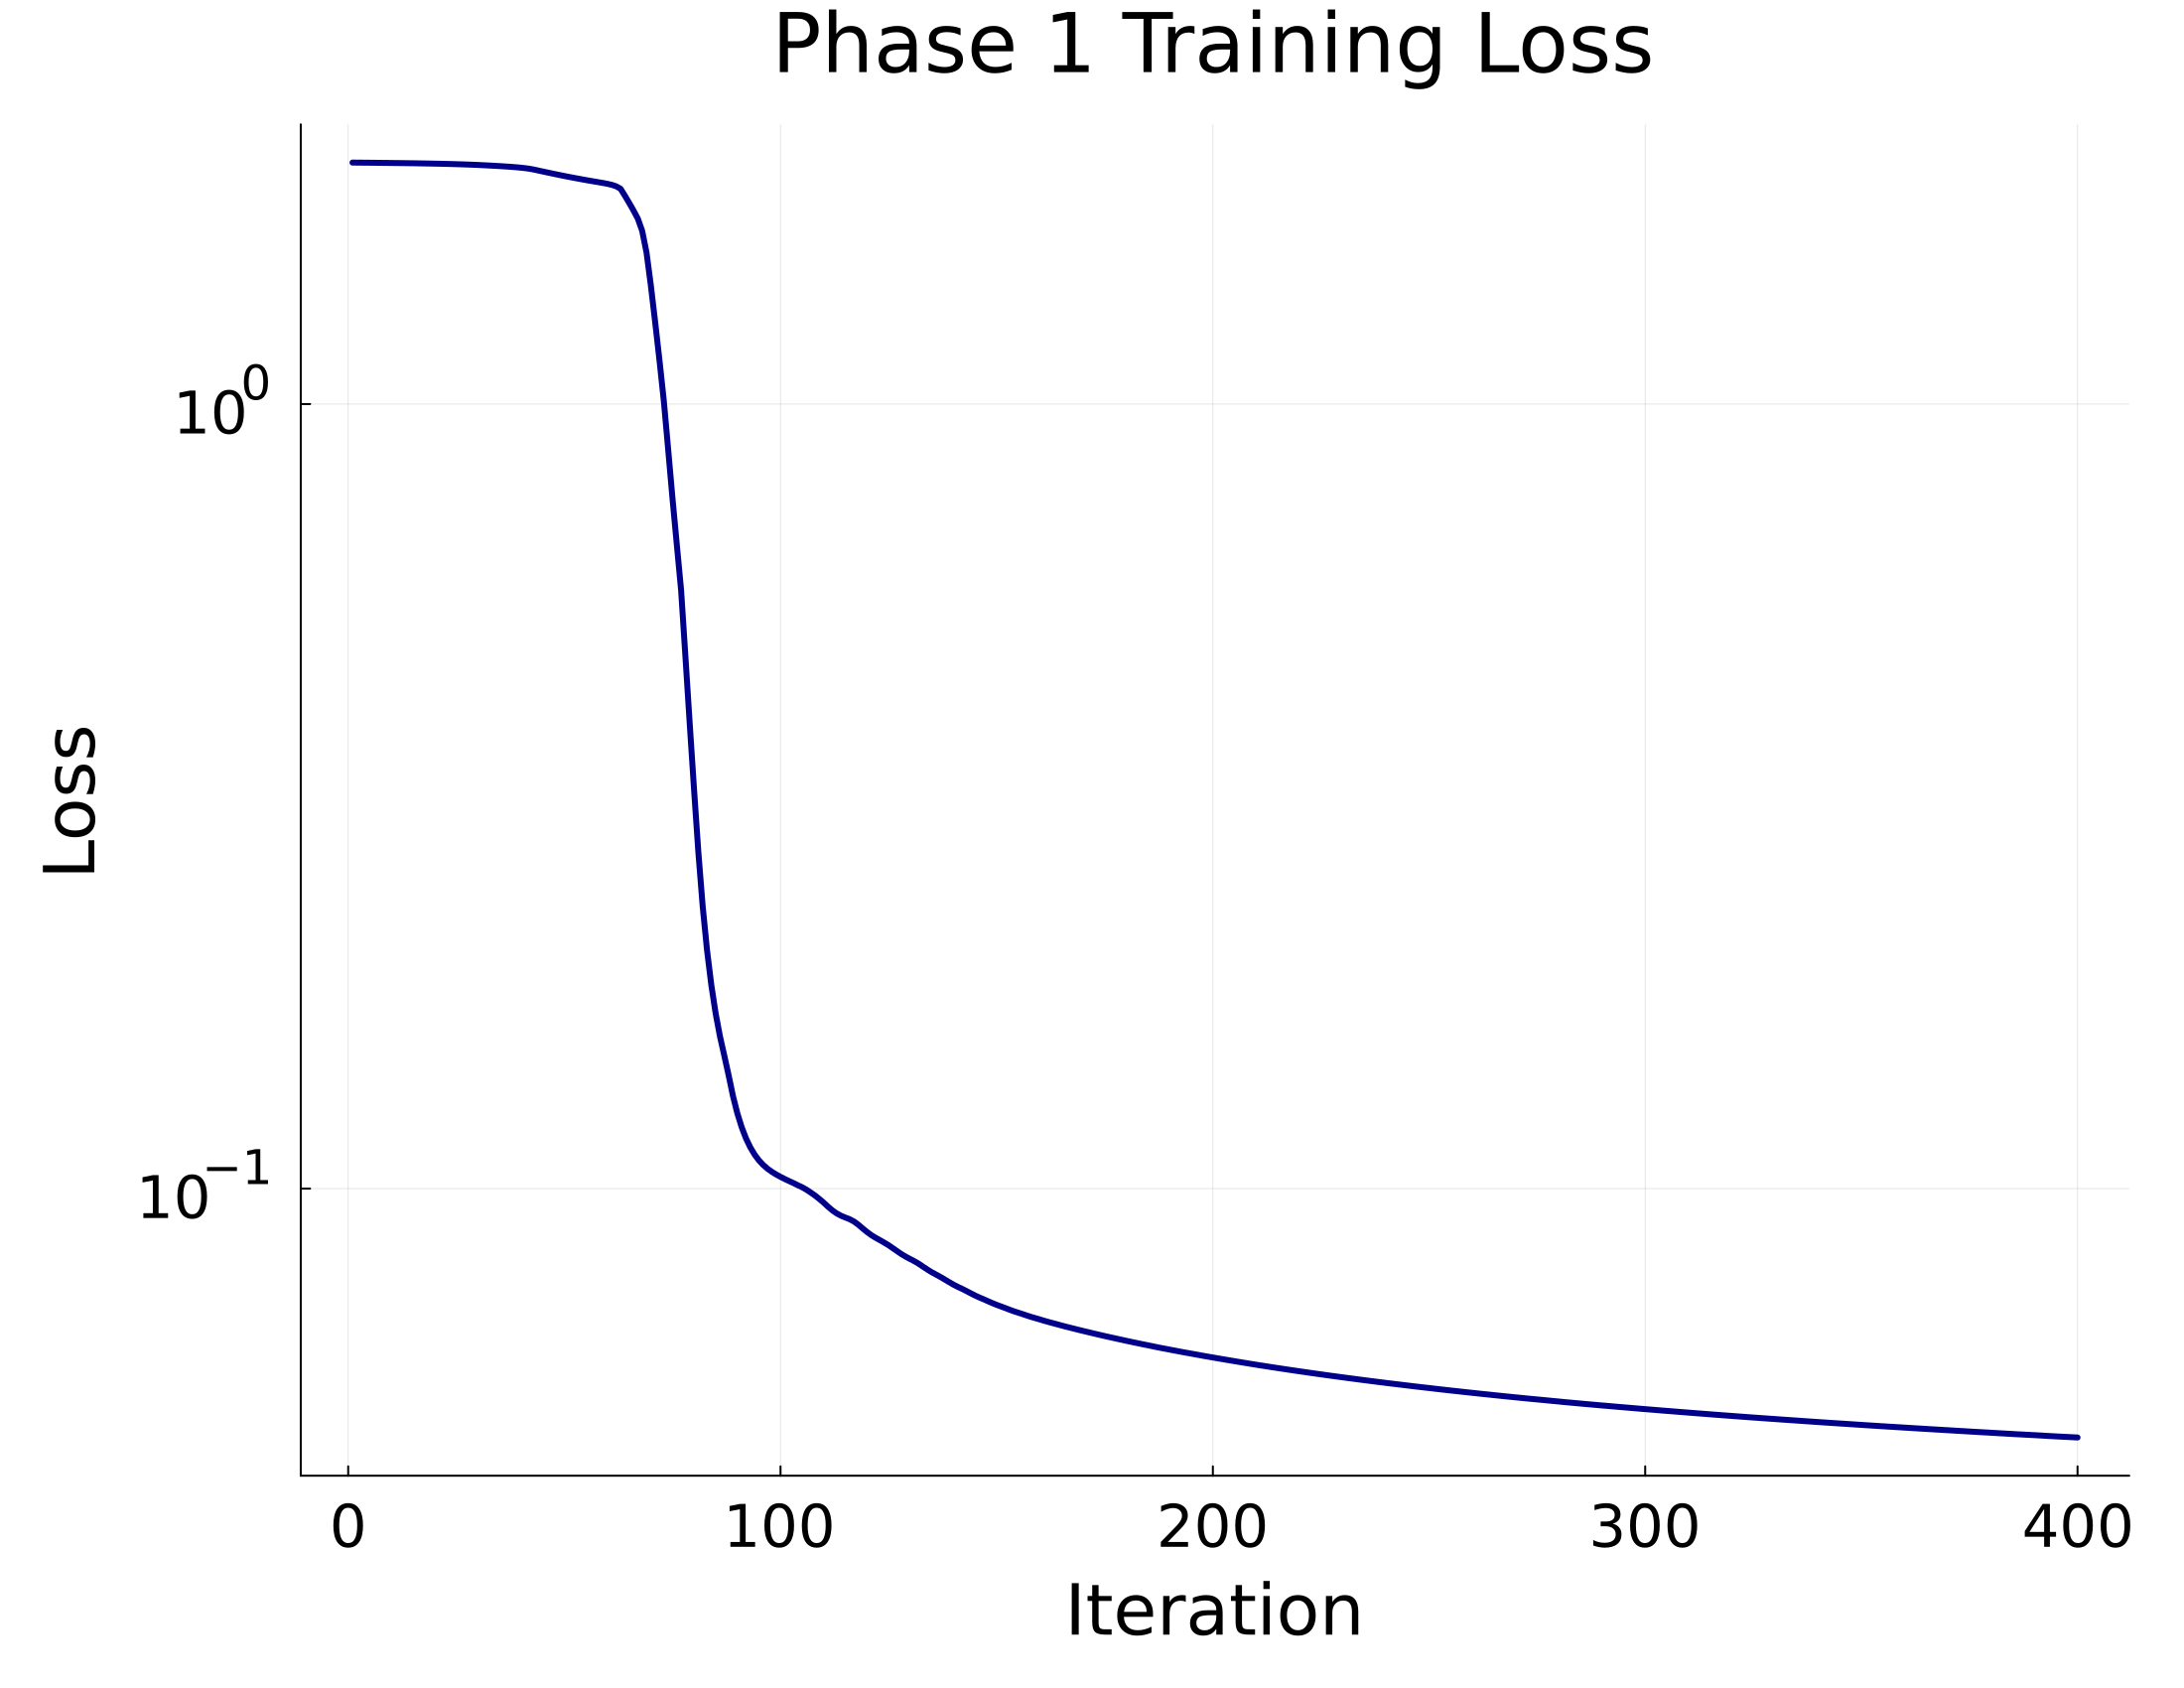
\includegraphics[width=\linewidth]{hybrid_training_loss.png}
\caption{Phase 1 training loss convergence through AdamW and L-BFGS phases.}
\label{fig:hybrid_training_loss}
\end{figure}

\begin{figure}[H]\centering
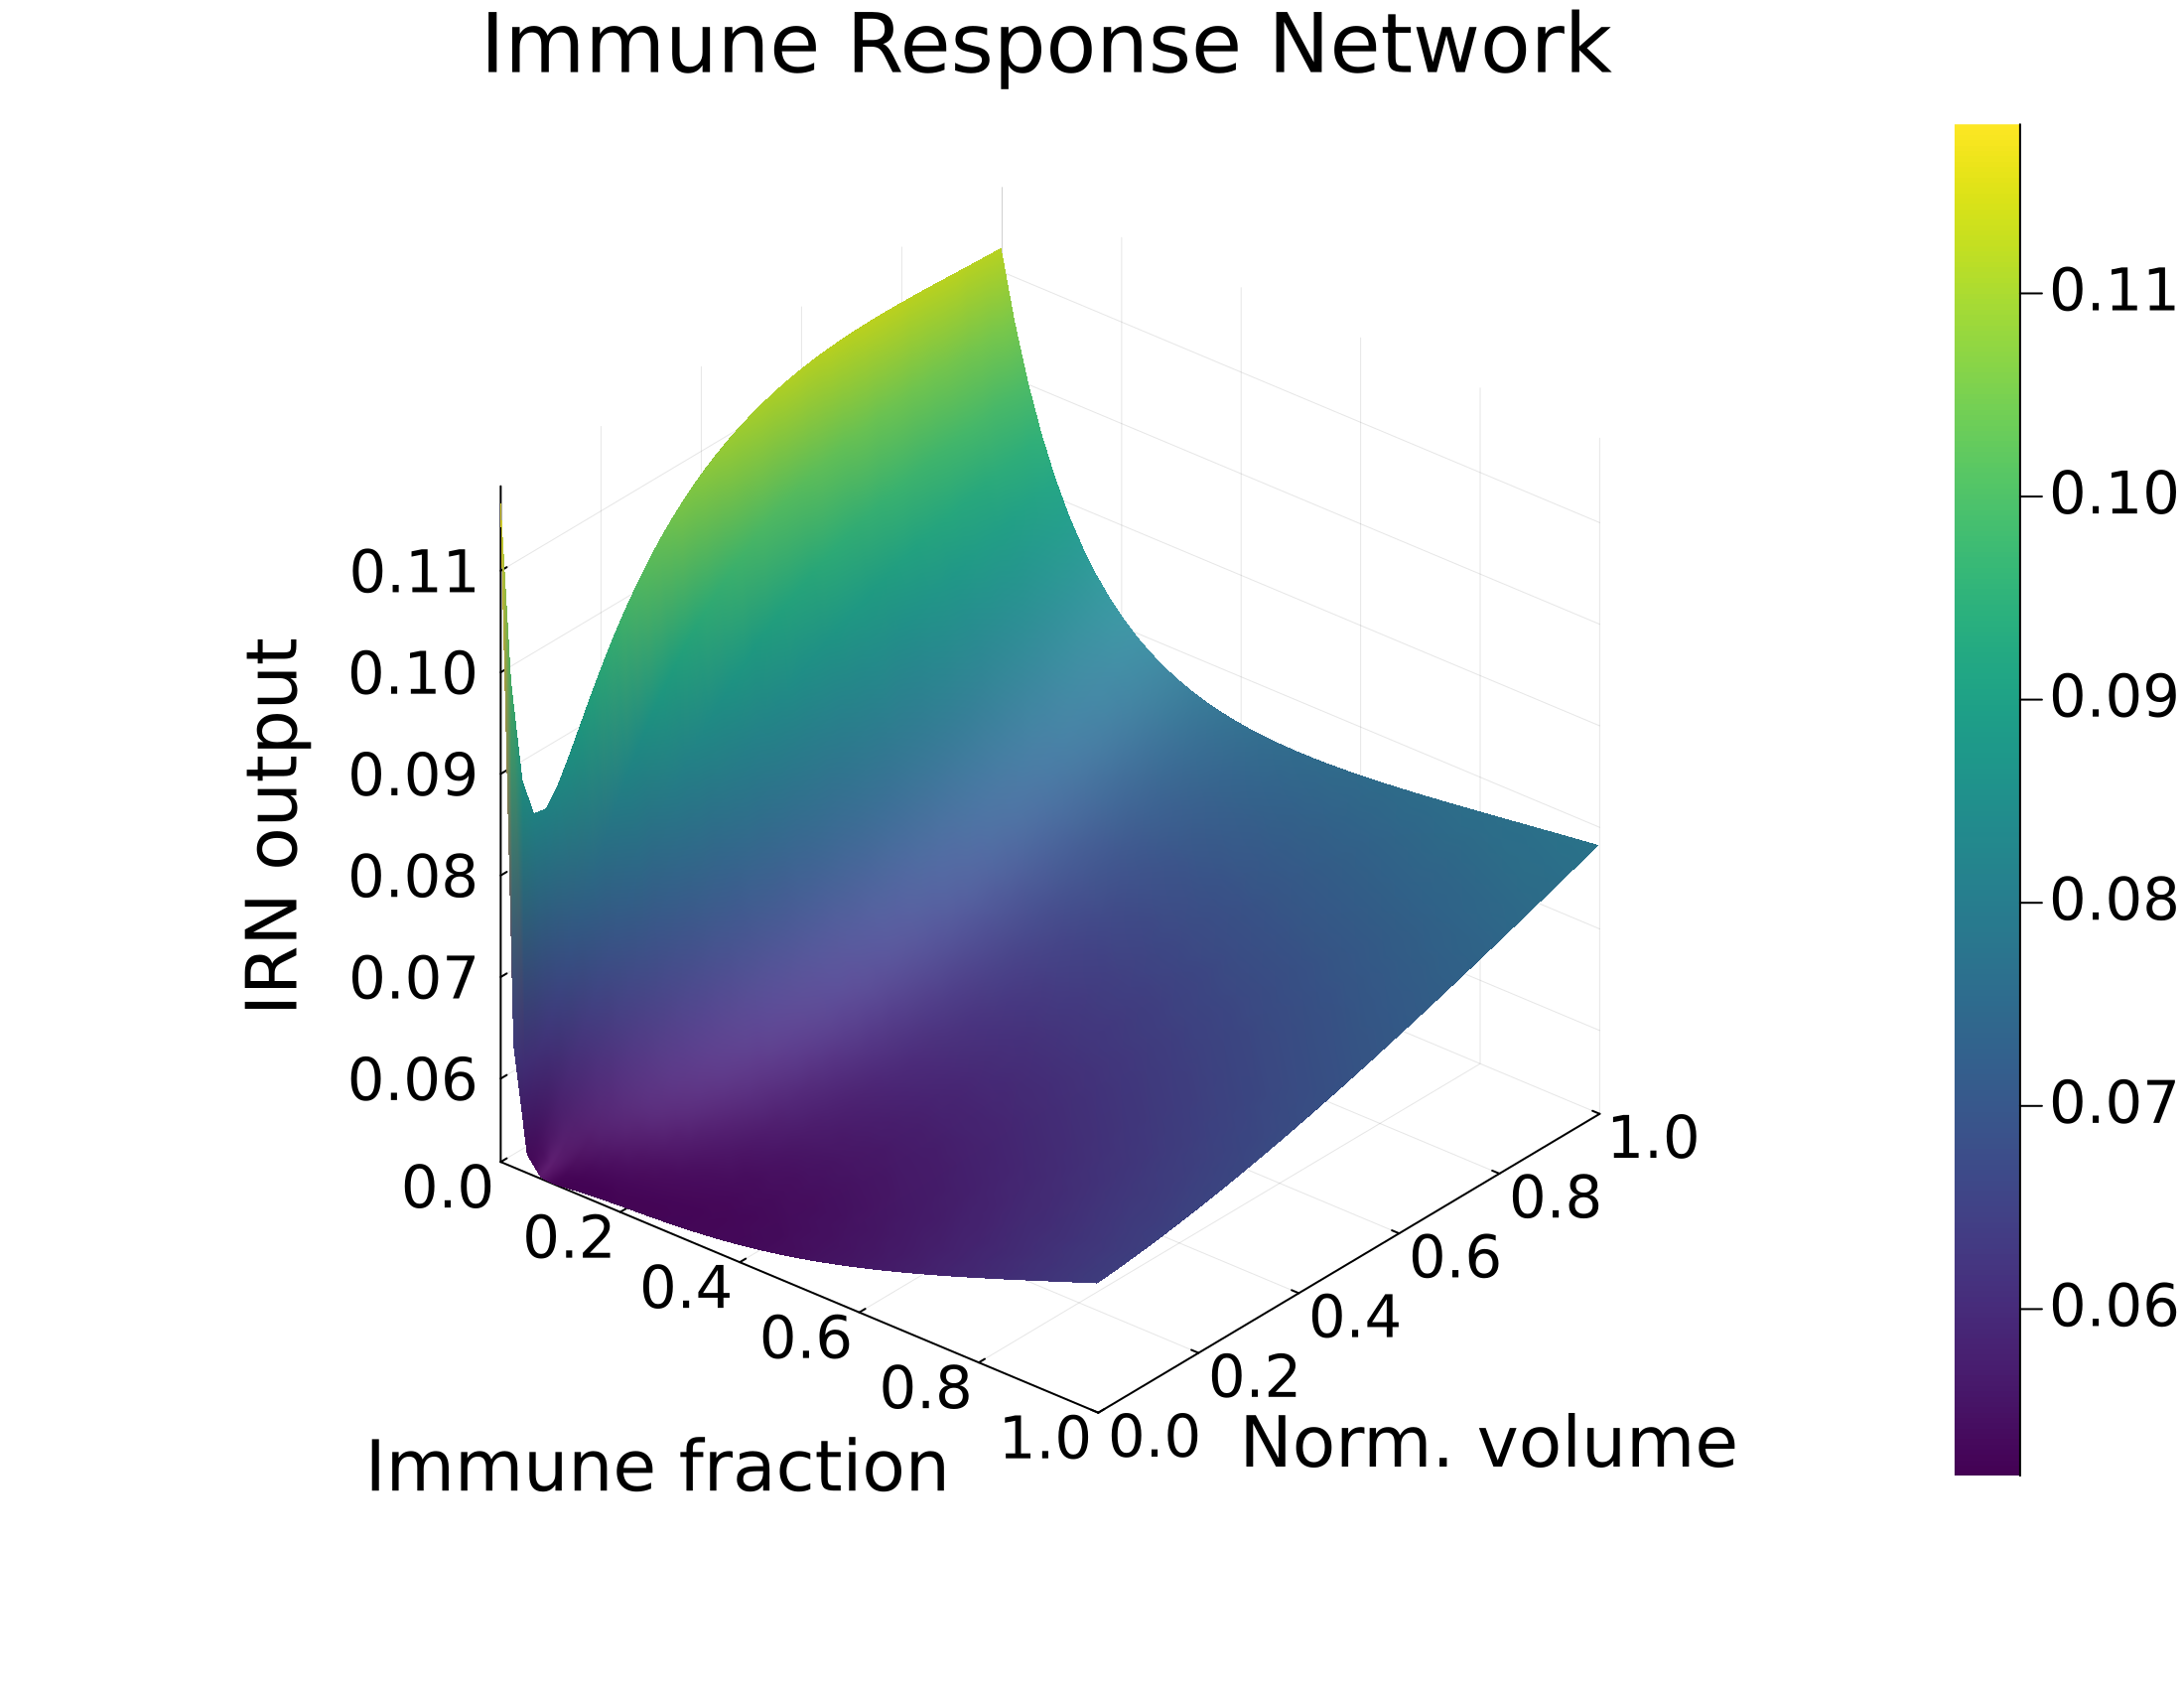
\includegraphics[width=\linewidth]{immune_network_surface.png}
\caption{Learned Immune Response Network surface showing volume-dependent activation and saturation behavior.}
\label{fig:irn_surface}
\end{figure}

\begin{figure}[H]\centering
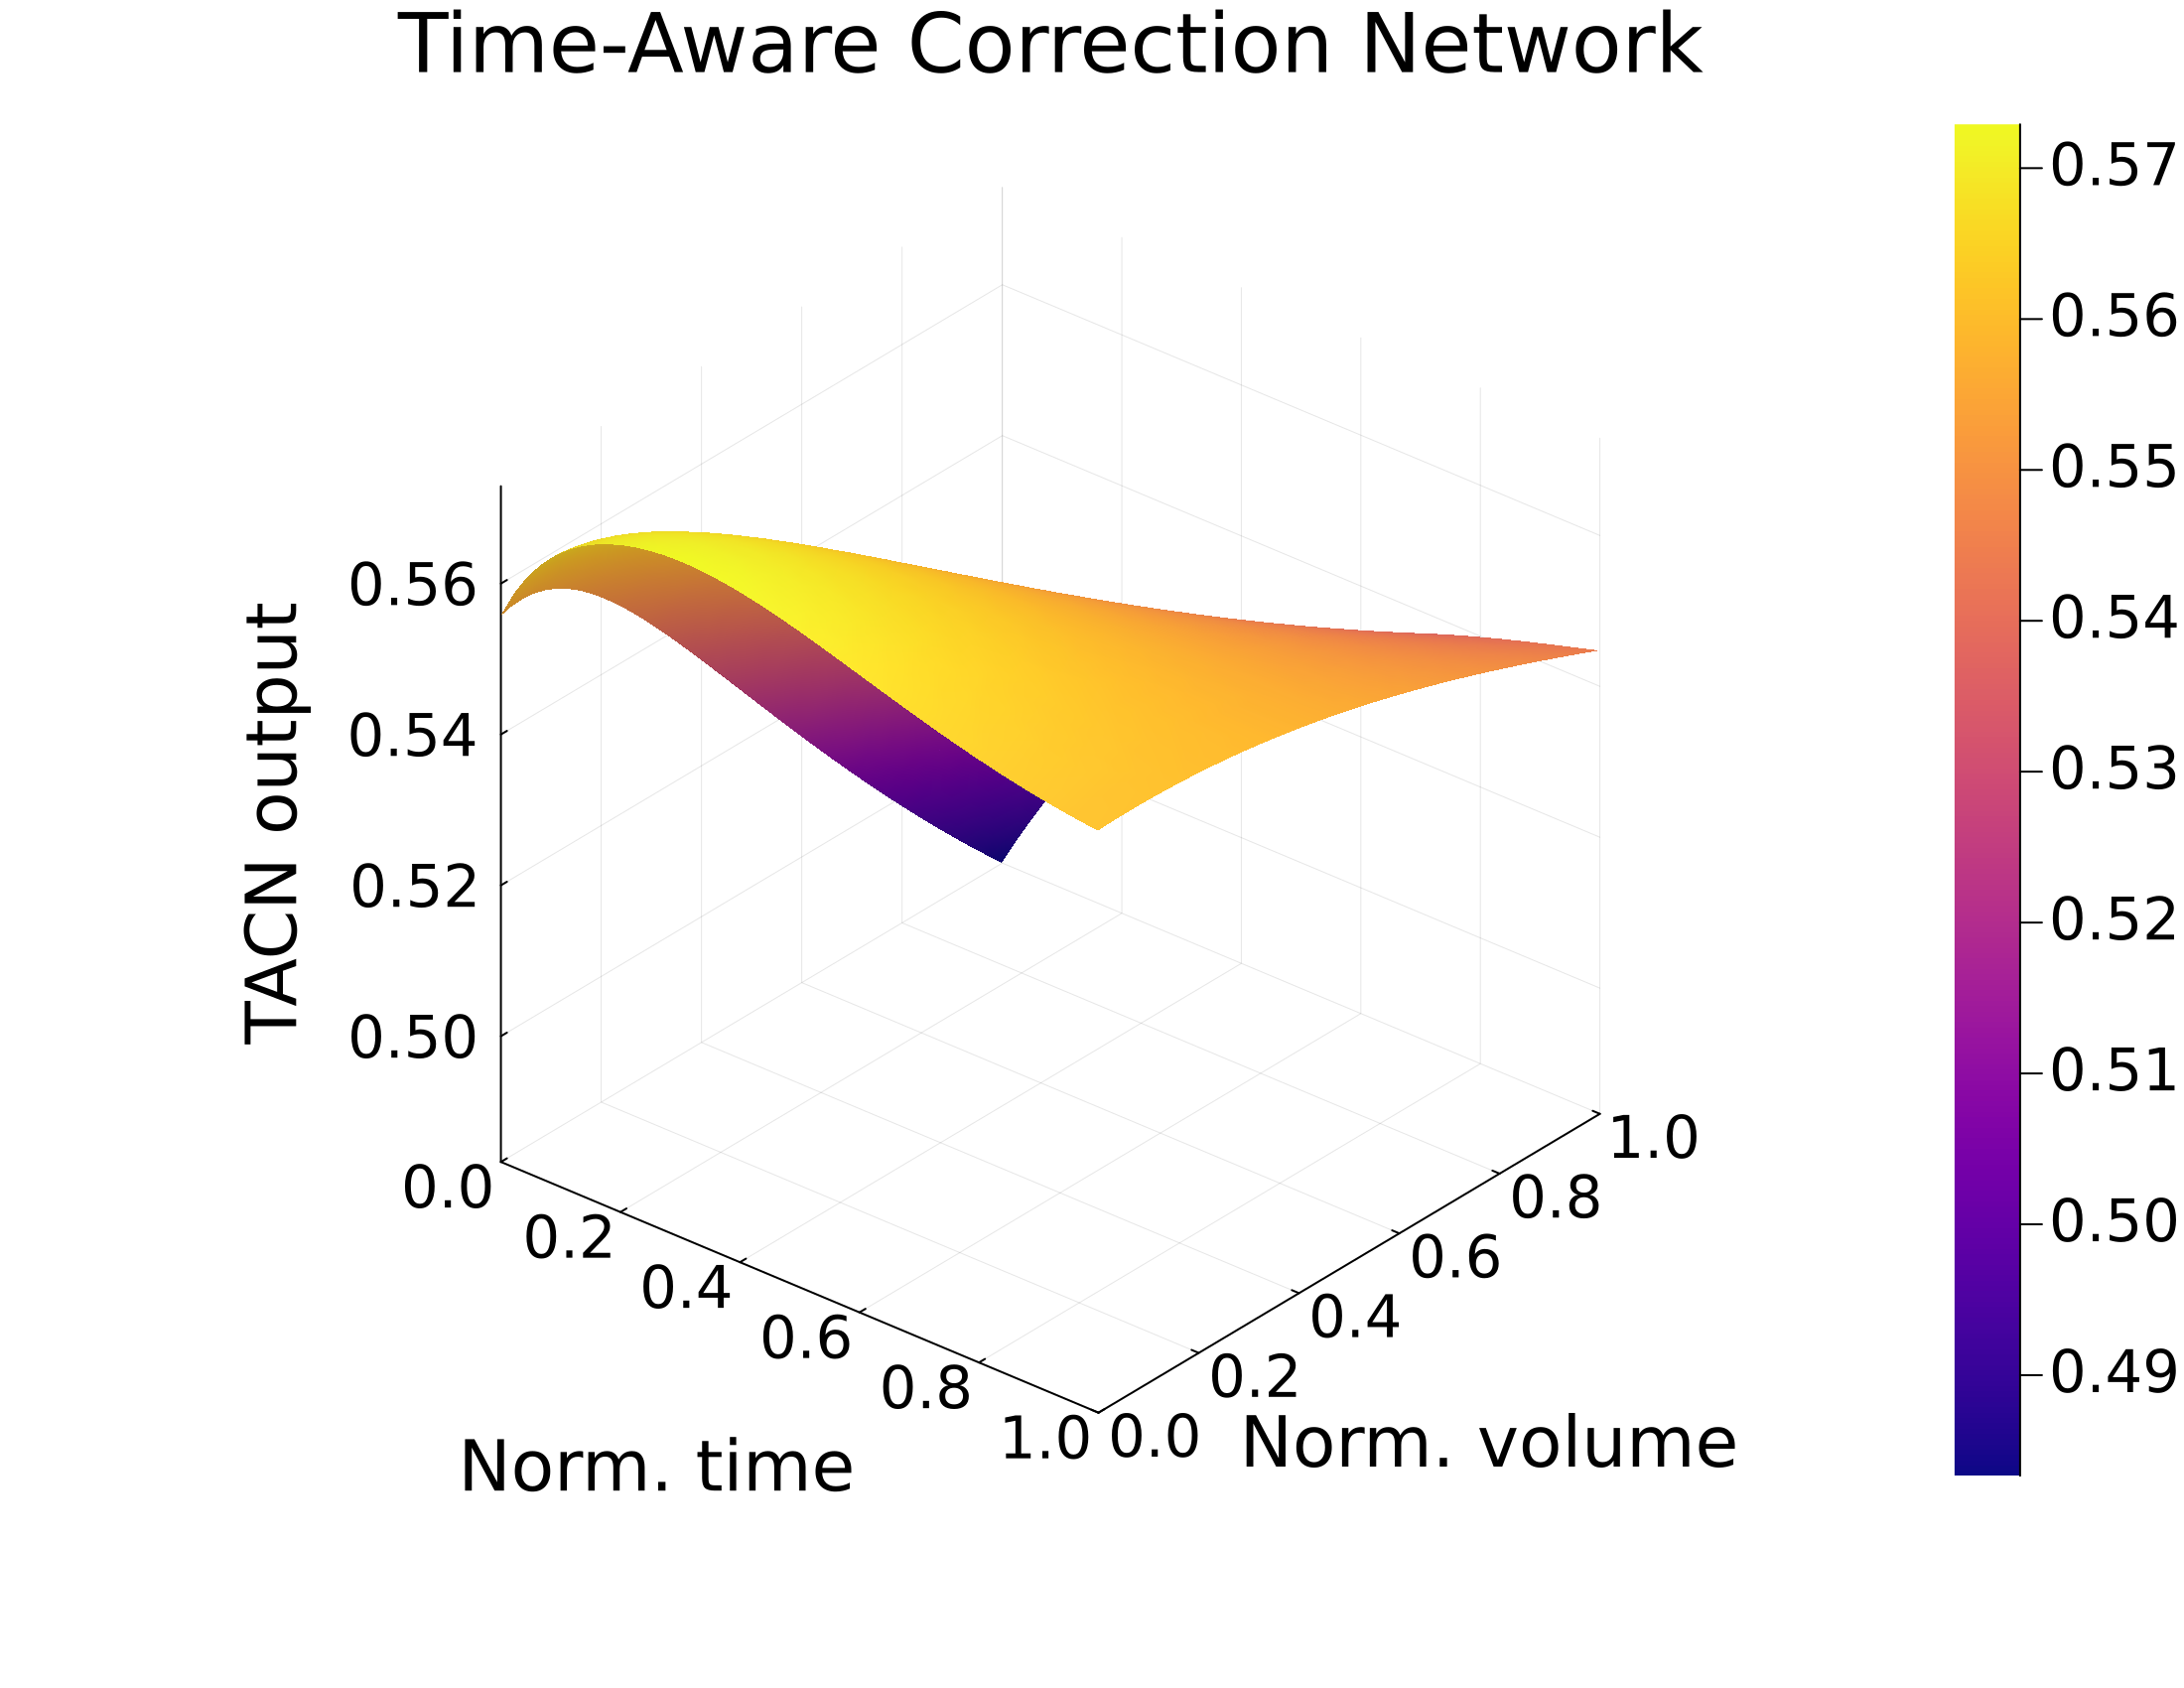
\includegraphics[width=\linewidth]{correction_network_surface.png}
\caption{Time-Aware Correction Network surface showing temporal adjustments.}
\label{fig:tacn_surface}
\end{figure}

\begin{figure}[H]\centering
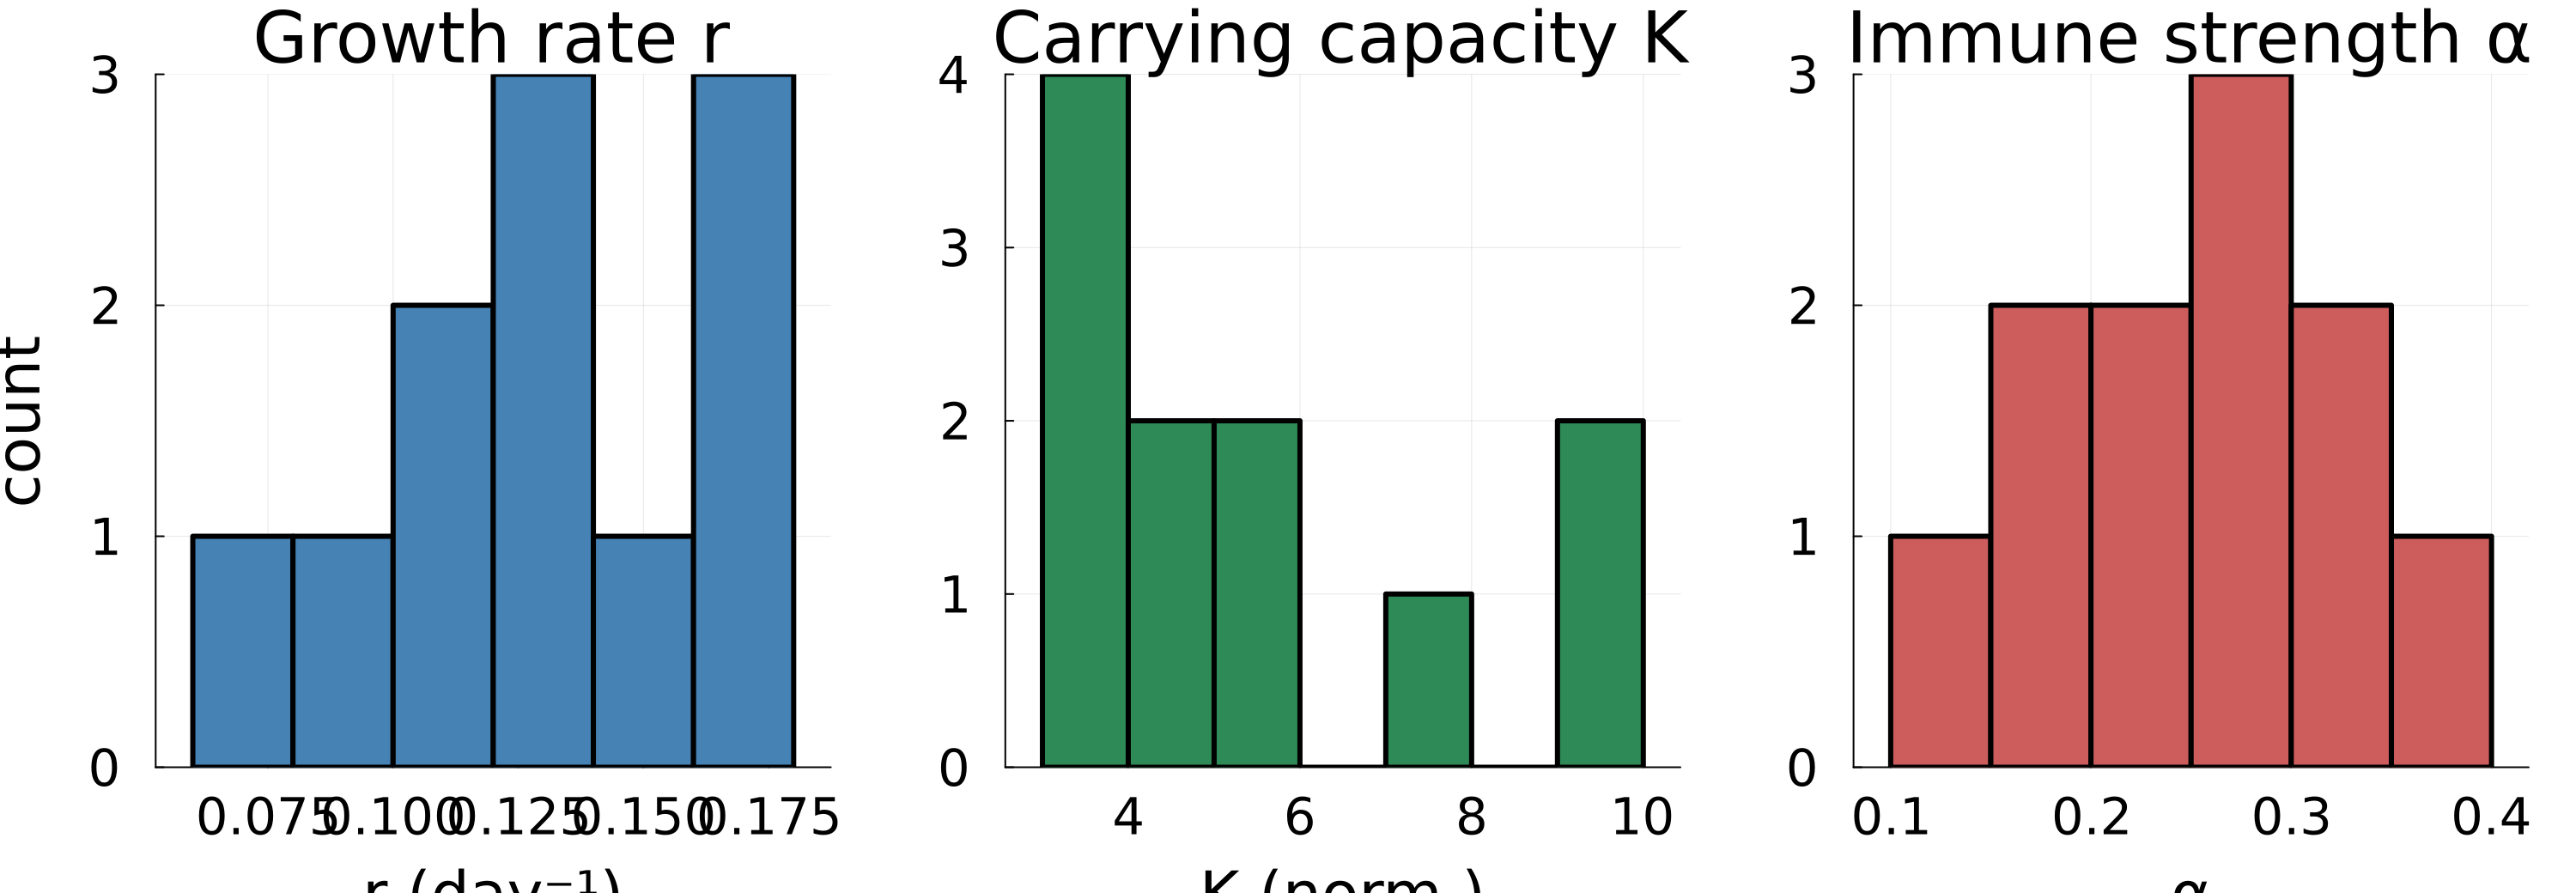
\includegraphics[width=\linewidth]{hybrid_param_distributions.png}
\caption{Distribution of learned parameters across tumor groups in the hybrid model.}
\label{fig:hybrid_params}
\end{figure}

\subsection{Phase 2: Structured-Parameter UDE}

The structured-parameter UDE achieves $R^2 = 0.991$ on training data (Figure~\ref{fig:pure_training_loss}), with strong correlation between predicted and observed volumes (Figure~\ref{fig:global_fit}). Figure~\ref{fig:group_vol_comparison} shows a representative case (C4$|$T2) where the model captures both immune-mediated suppression and growth dynamics; the separation between immune-present and immune-absent trajectories demonstrates biological consistency. Component decomposition (Figure~\ref{fig:components}) reveals Gompertz growth dominating early phases with immune killing peaking around days 15--20.

\begin{figure}[H]\centering
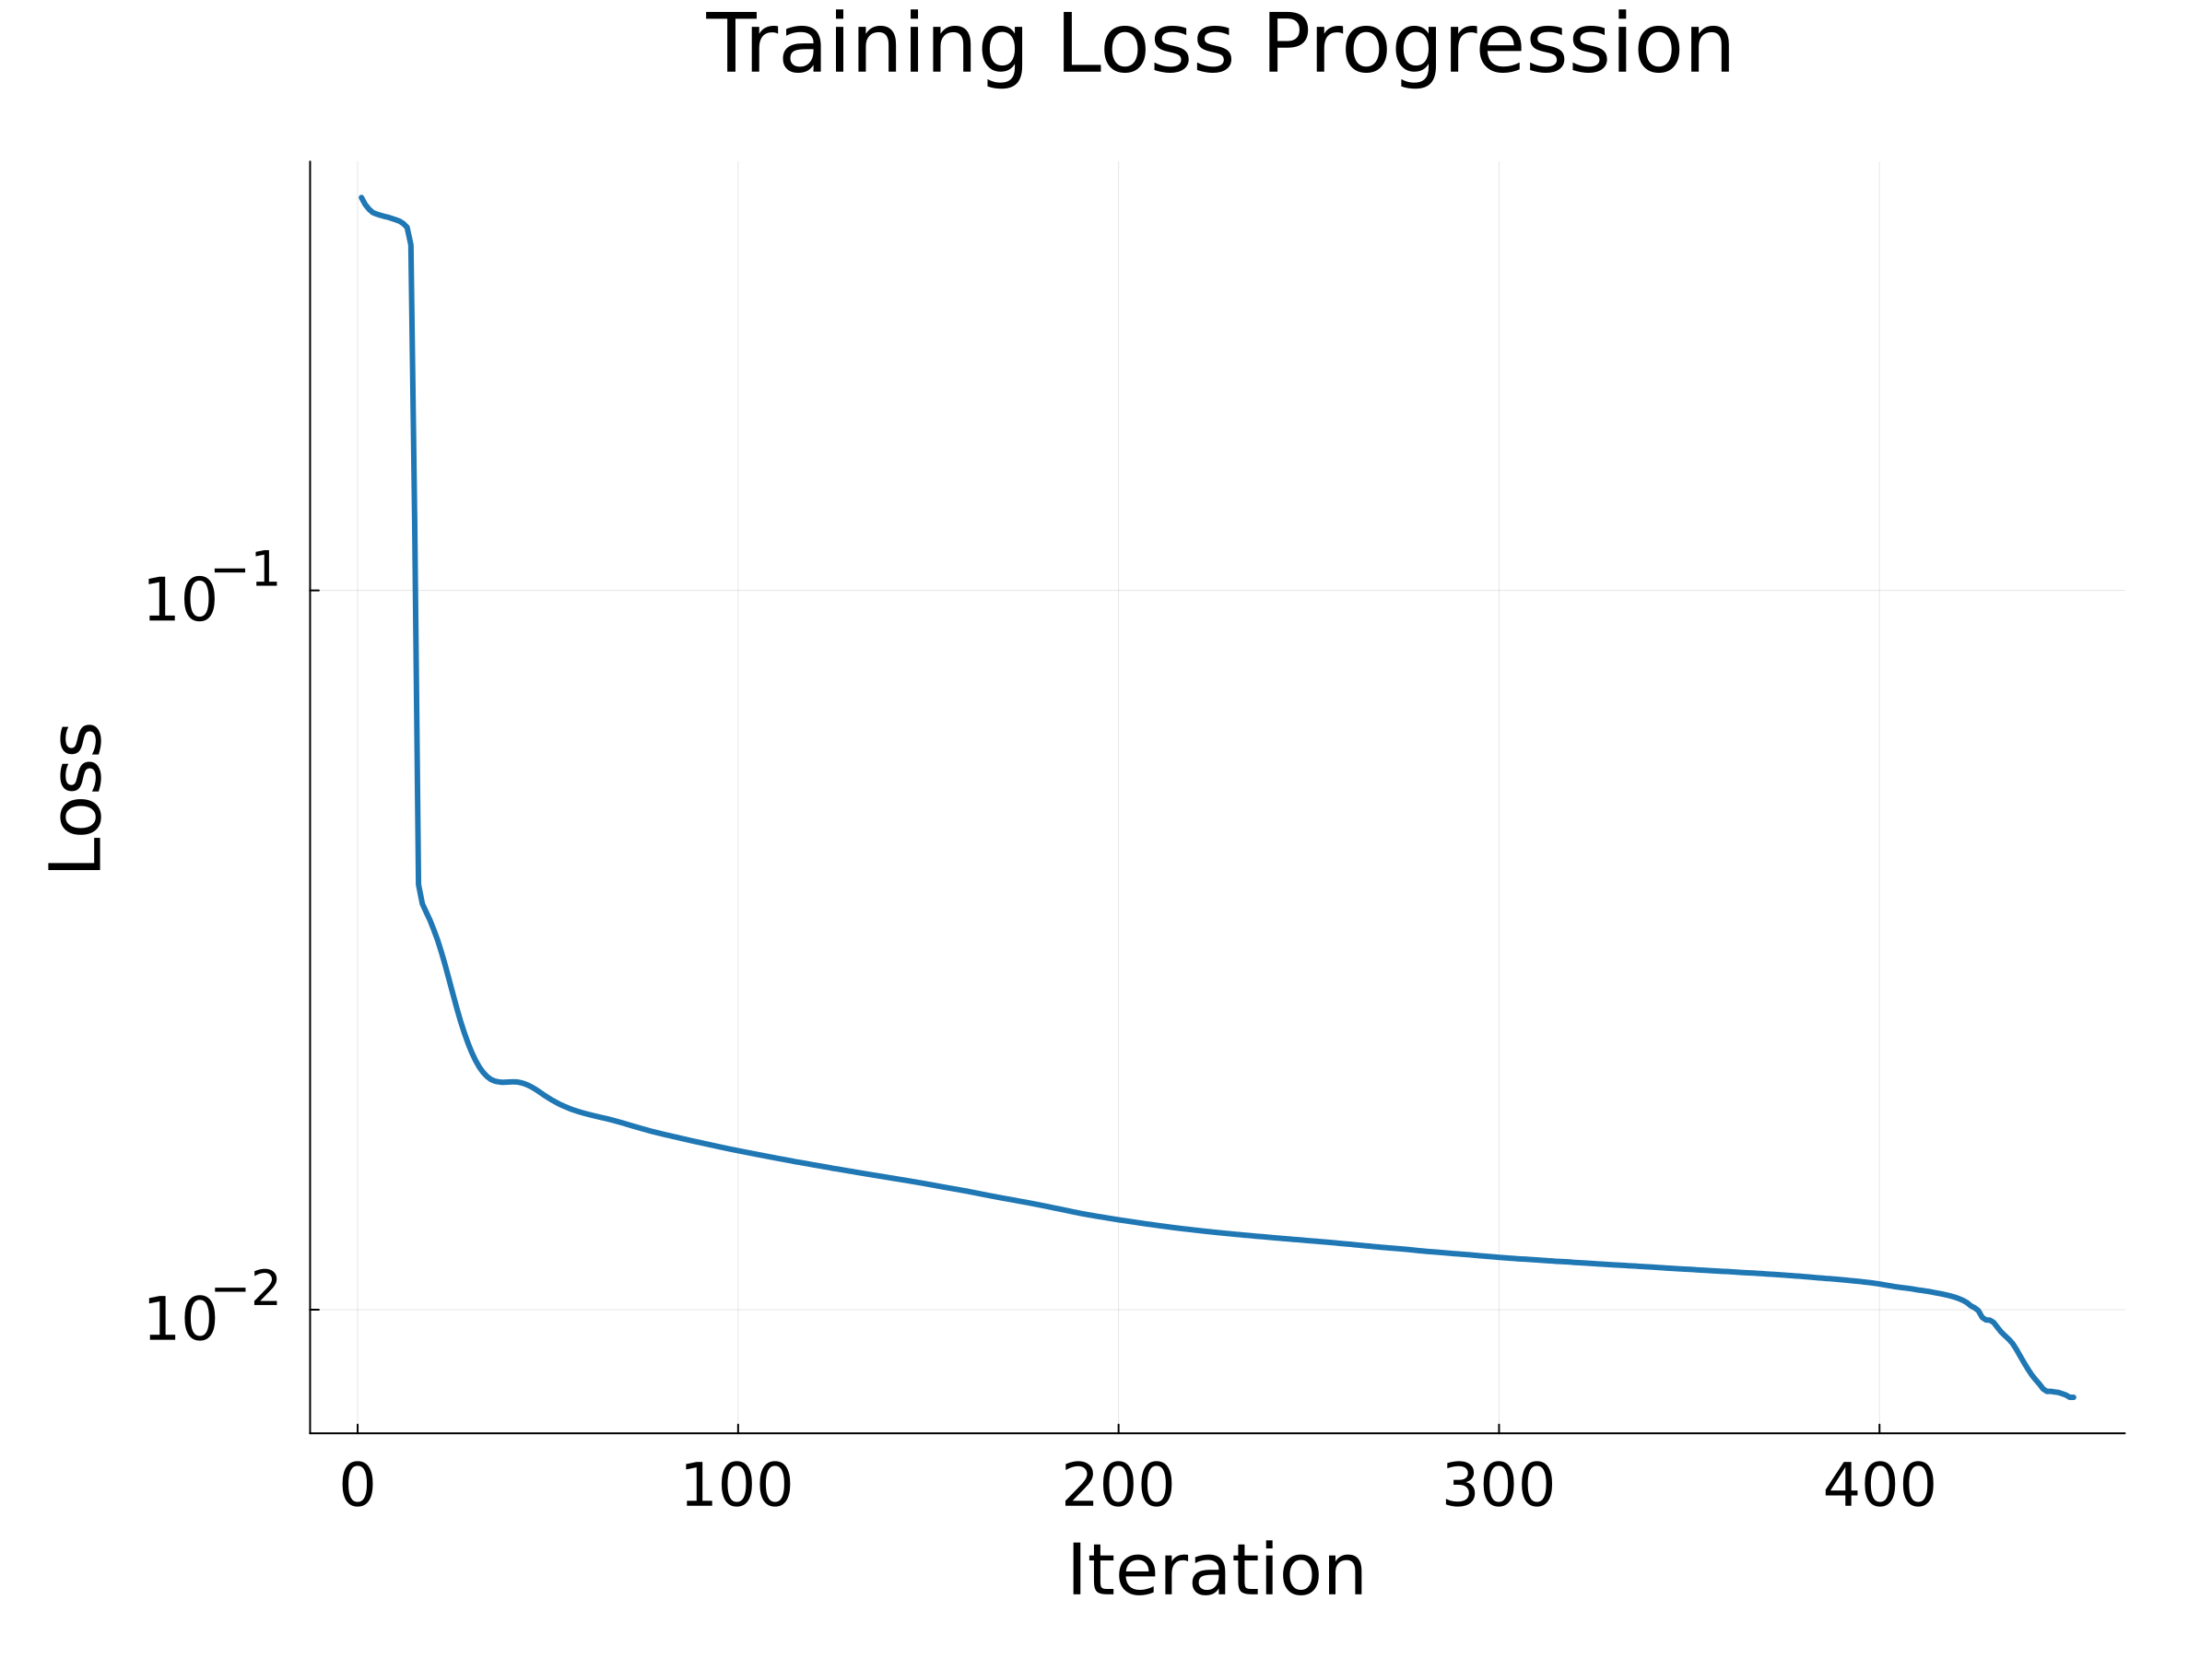
\includegraphics[width=\linewidth]{pure_training_loss.png}
\caption{Phase 2 training loss showing convergence to lower loss than Phase 1.}
\label{fig:pure_training_loss}
\end{figure}

\begin{figure}[H]\centering
\includegraphics[width=\linewidth]{global_fit.png}
\caption{Global fit for the structured-parameter UDE ($R^2 = 0.991$).}
\label{fig:global_fit}
\end{figure}

\begin{figure}[H]\centering
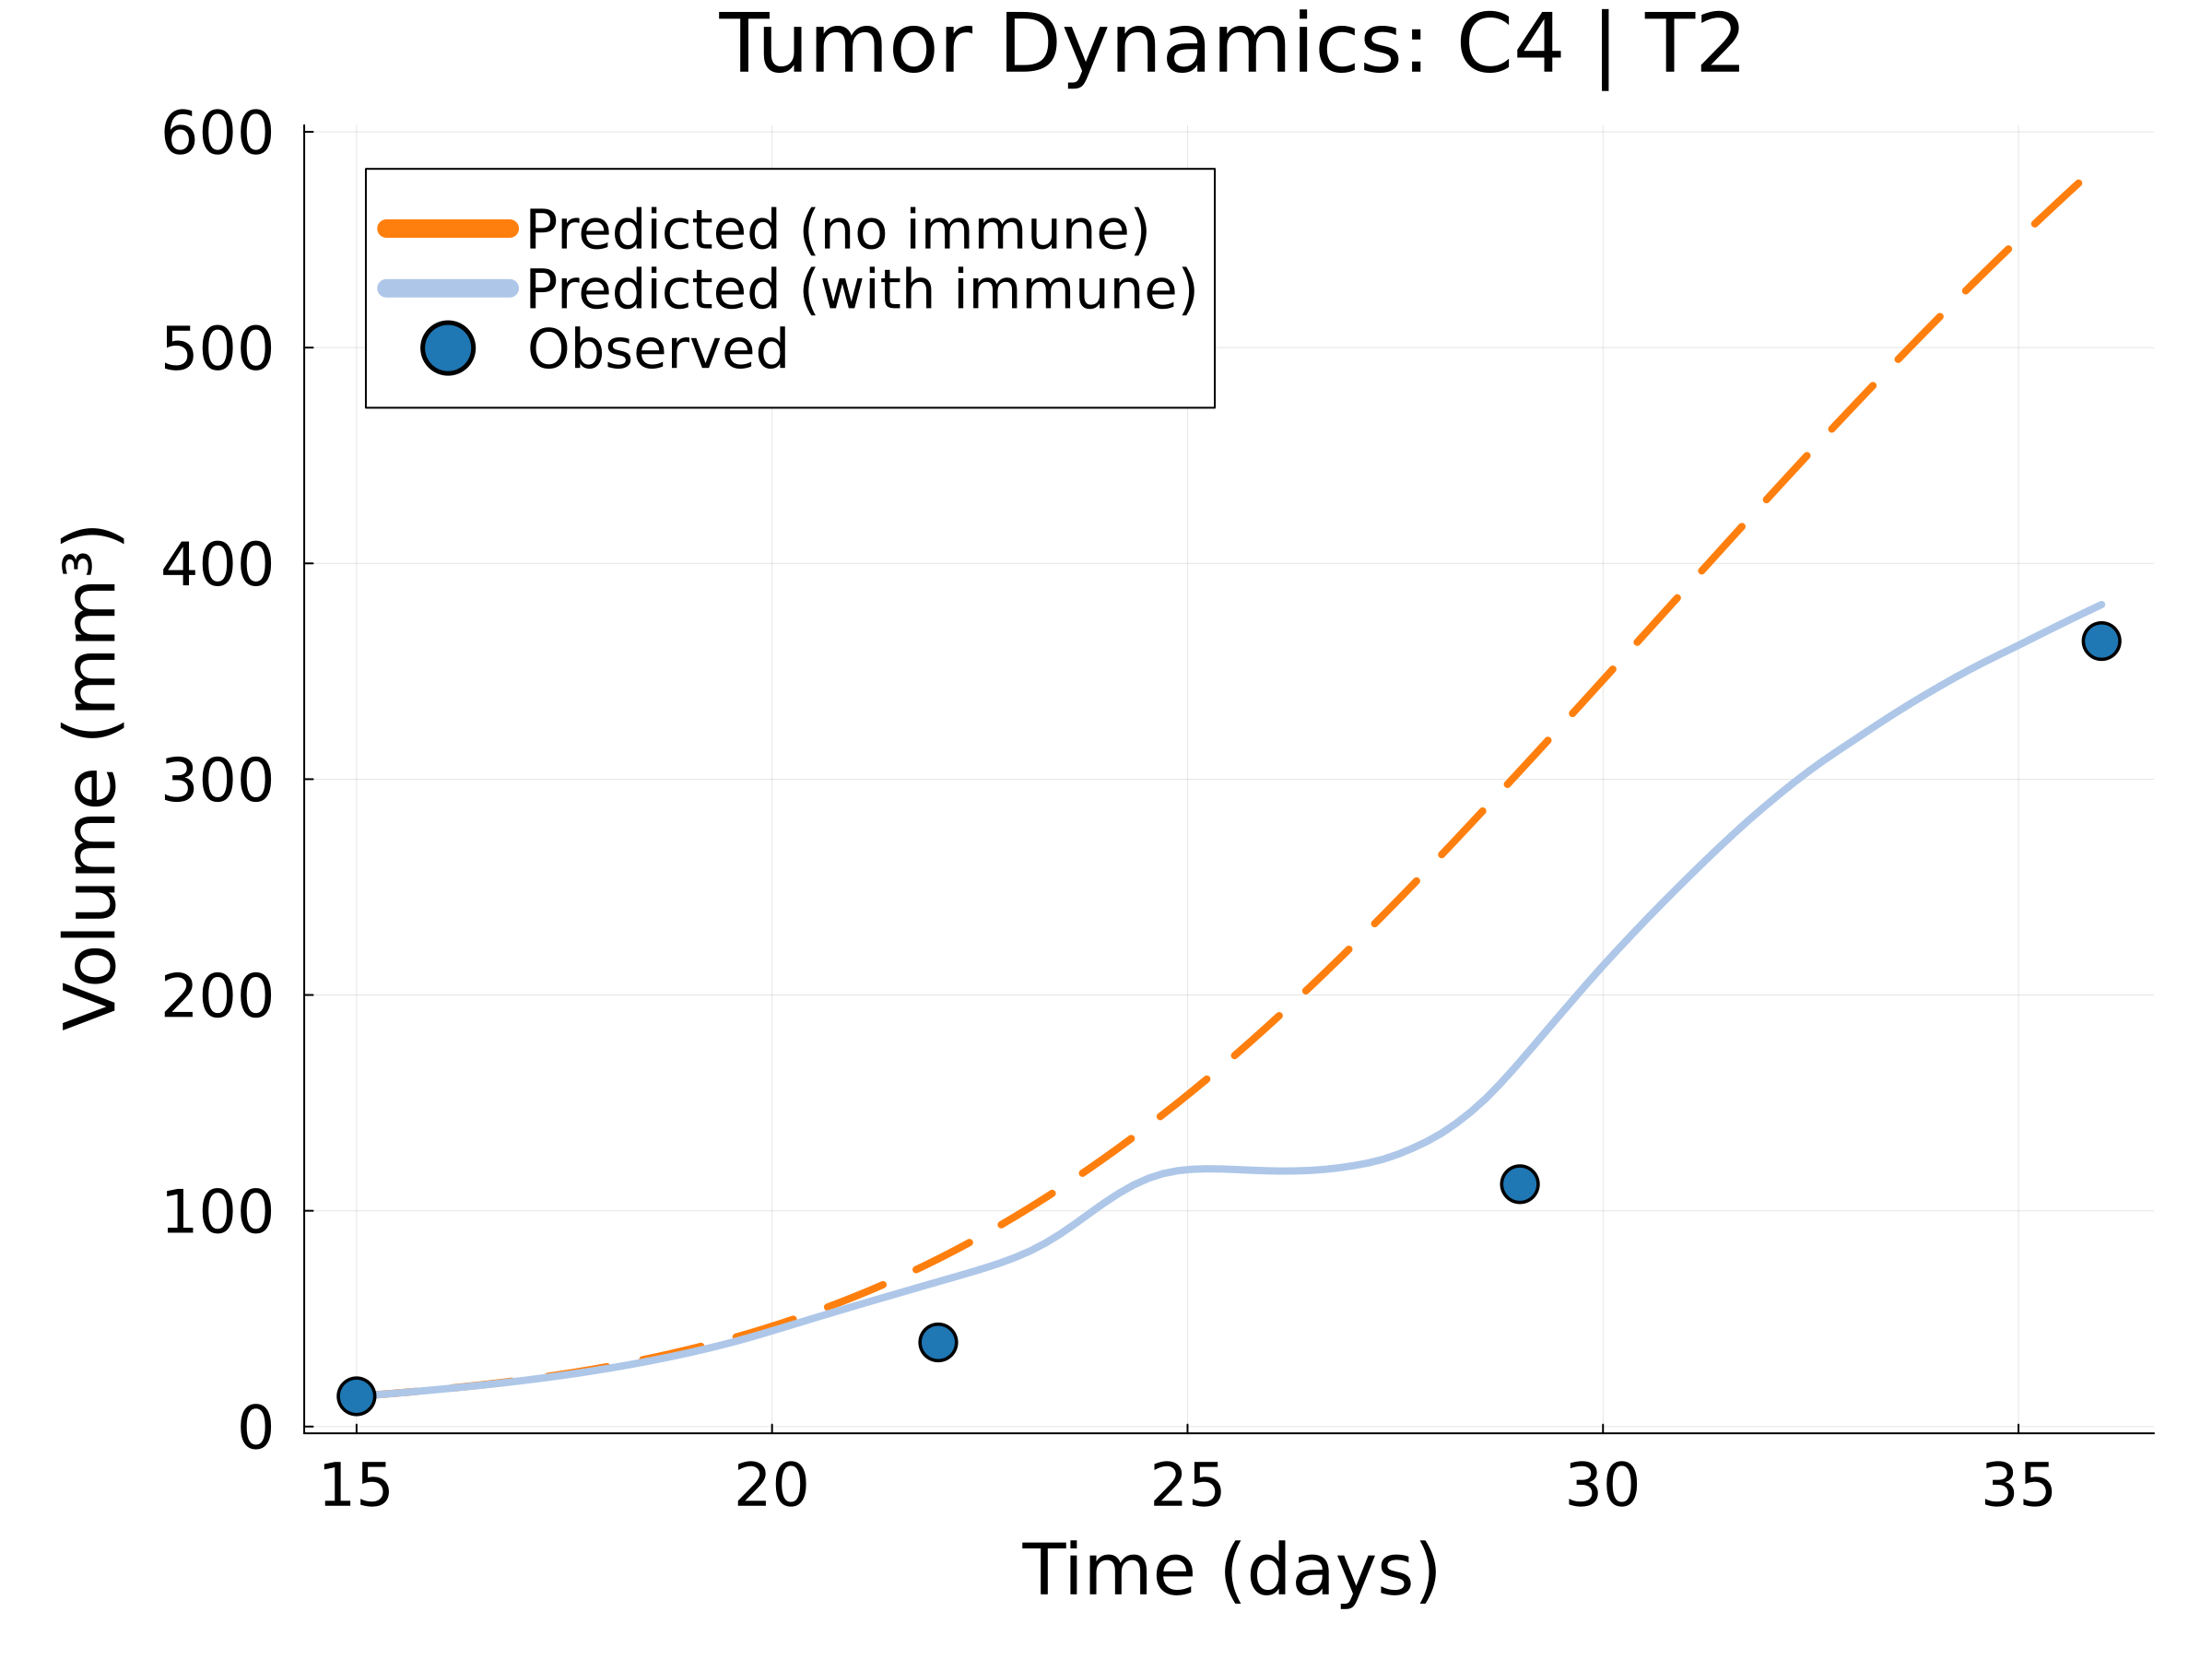
\includegraphics[width=\linewidth]{group_C4_T2_volume_comparison.png}
\caption{Representative group (C4$|$T2) showing observed data, predicted trajectories, and counterfactual predictions without immune influence.}
\label{fig:group_vol_comparison}
\end{figure}

\begin{figure}[H]\centering
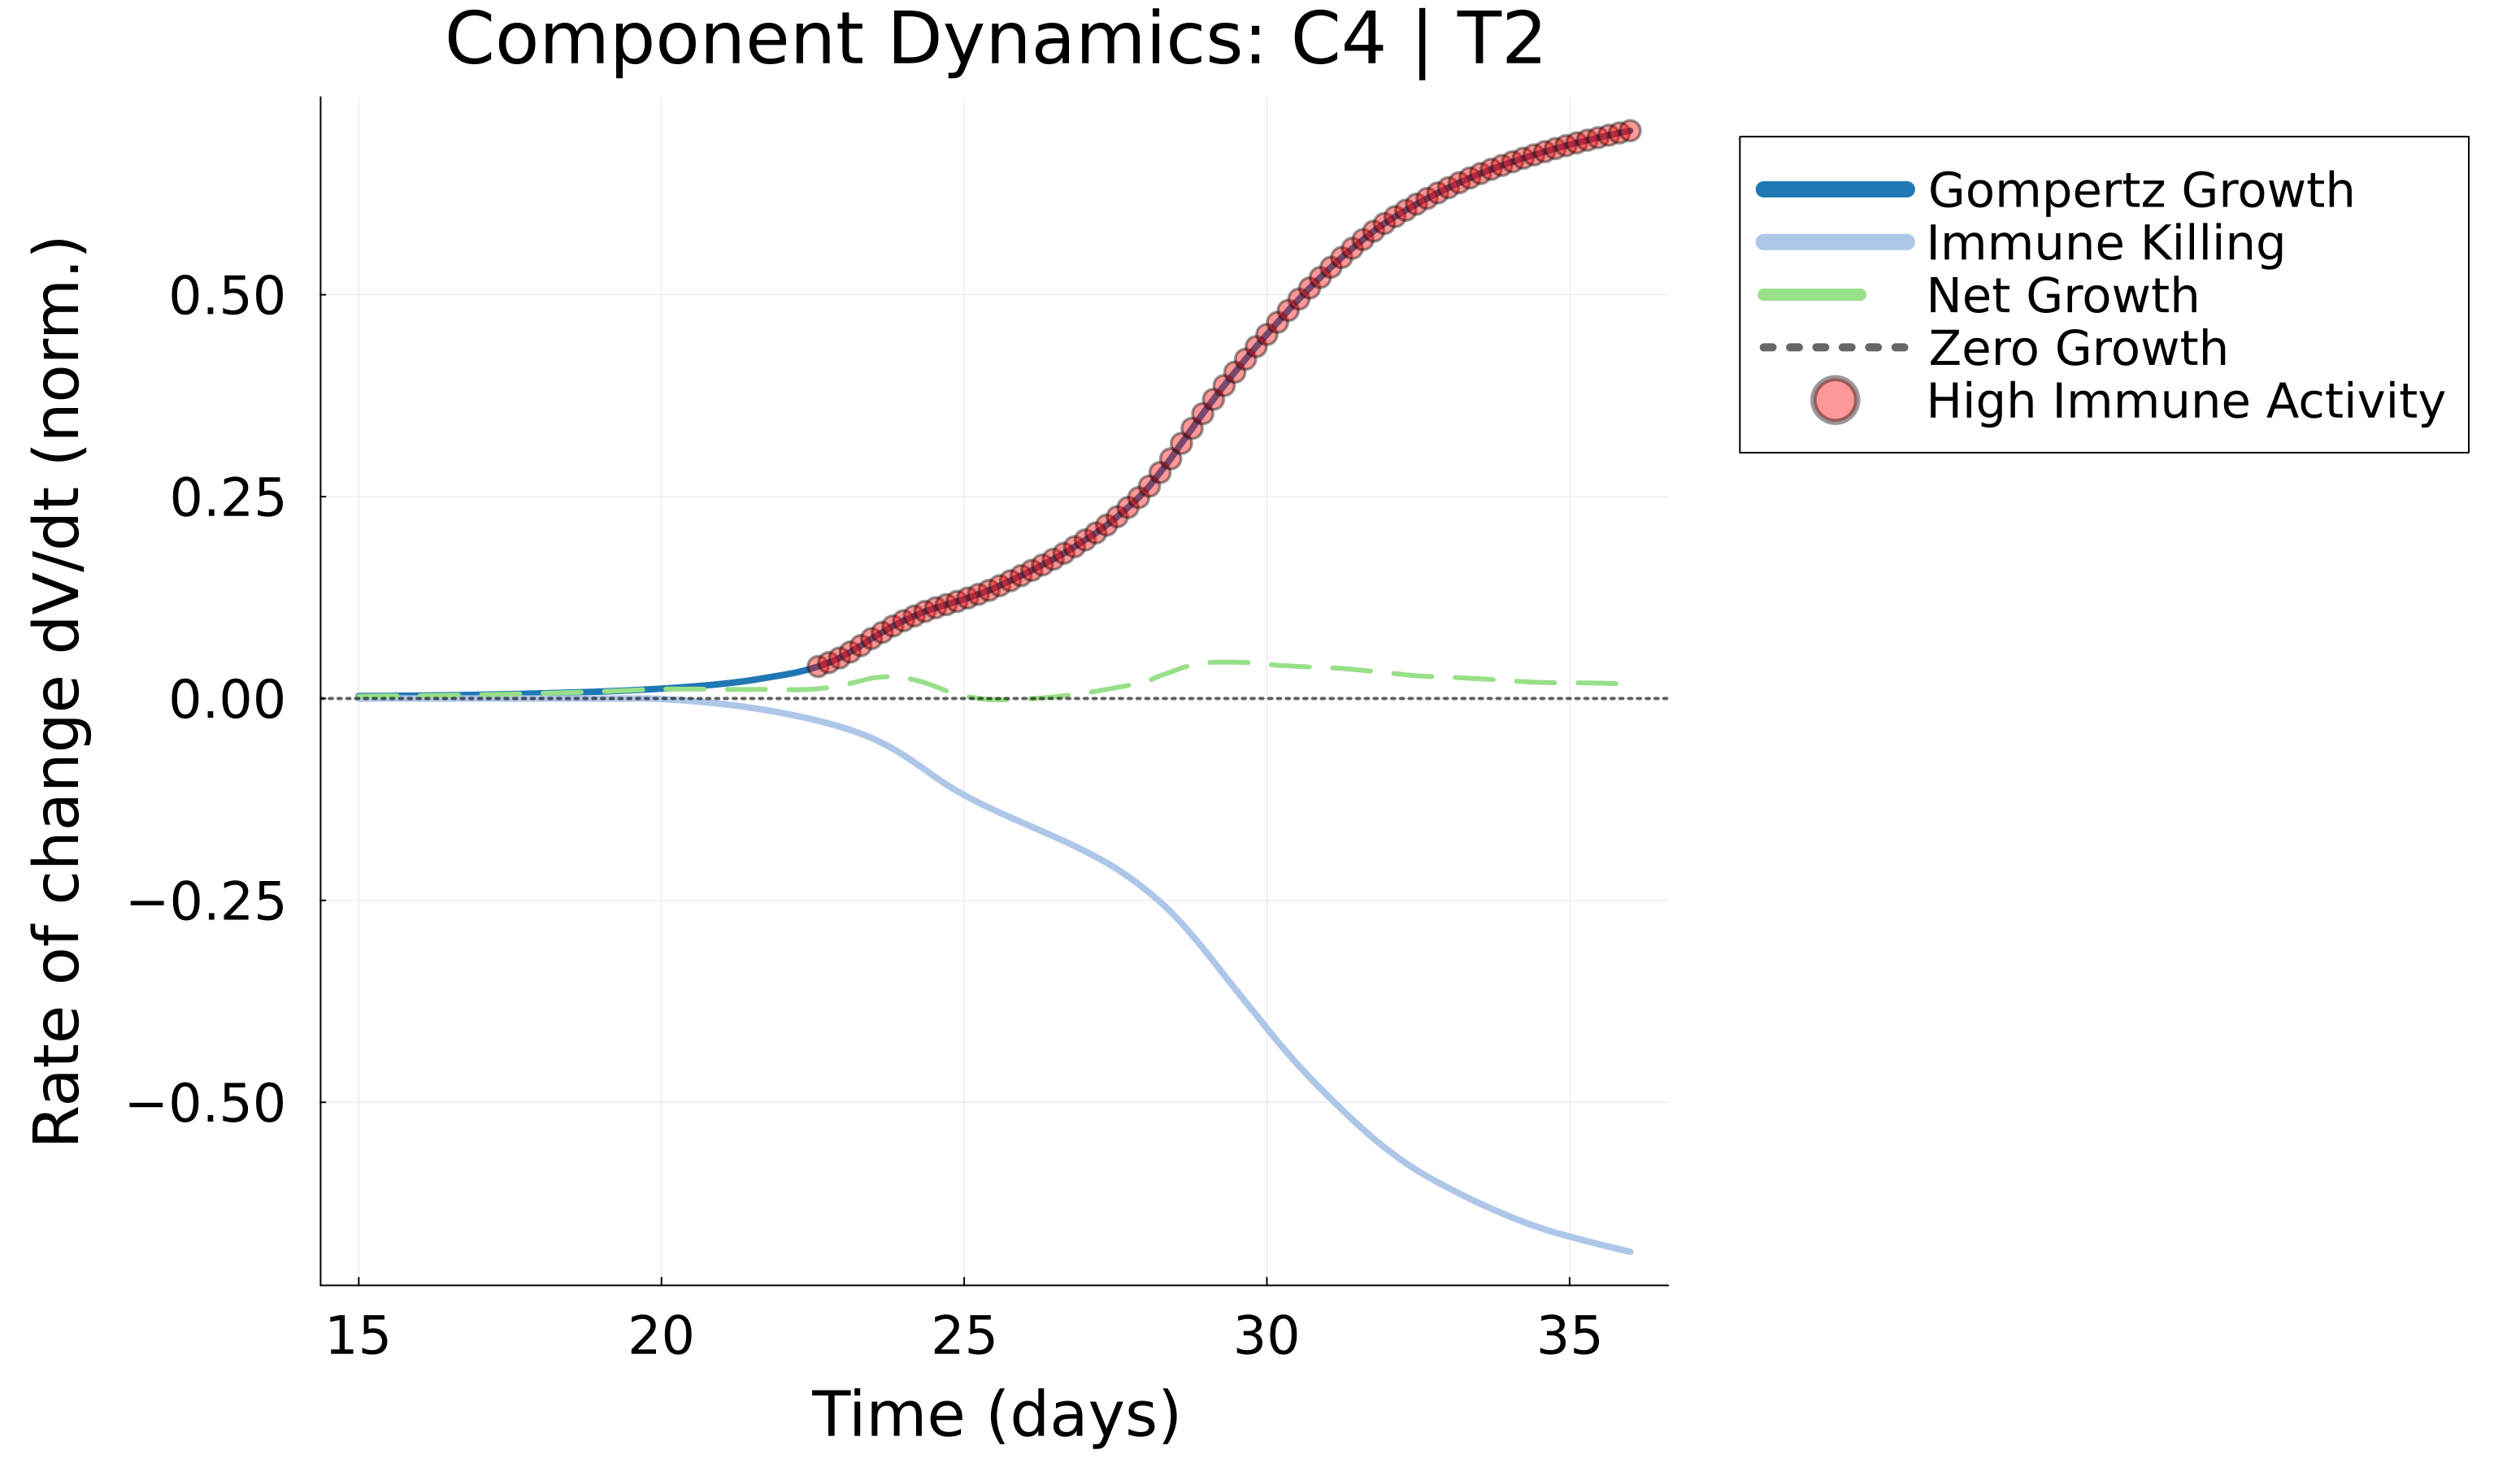
\includegraphics[width=\linewidth]{group_C4_T2_component_dynamics.png}
\caption{Component dynamics for C4$|$T2: Gompertz growth, immune killing, and net growth.}
\label{fig:components}
\end{figure}

\subsection{Cross-Validation and Forecasting}

Table~\ref{tab:cv_metrics} reports cross-validation metrics across all five held-out groups. The structured-parameter UDE achieves mean $R^2 = 0.945$ (std $= 0.034$) and mean sMAPE $= 8.3\%$, indicating robust generalization.

\begin{table}[H]\centering
\small
\begin{tabular}{@{}lccccc@{}}
\toprule
\textbf{Group} & \textbf{MAE} & \textbf{RMSE} & \textbf{sMAPE} & \textbf{R\textsuperscript{2}} & \textbf{Final Vol. Err.} \\
& \textbf{(mm\textsuperscript{3})} & \textbf{(mm\textsuperscript{3})} & \textbf{(\%)} & & \textbf{(\%)} \\
\midrule
C2-T1 & 30.5 & 30.5 & 16.8 & 0.909 & 16.8 \\
C2-T2 & 17.2 & 17.2 & 8.4 & 0.915 & 8.4 \\
C2-T3 & 8.7 & 8.7 & 6.7 & 0.947 & 6.7 \\
C2-T4 & 0.9 & 0.9 & 1.1 & 0.958 & 1.1 \\
C4-T5 & 16.5 & 16.5 & 8.7 & 0.998 & 8.7 \\
\midrule
\textbf{Mean} & \textbf{14.8} & \textbf{14.8} & \textbf{8.3} & \textbf{0.945} & \textbf{8.3} \\
\textbf{Std} & \textbf{11.4} & \textbf{11.4} & \textbf{5.7} & \textbf{0.034} & \textbf{5.7} \\
\bottomrule
\end{tabular}
\caption{Cross-validation metrics for the structured-parameter UDE across held-out groups.}
\label{tab:cv_metrics}
\end{table}

Figures~\ref{fig:c4t5_forecast}--\ref{fig:c4t5_long_forecast} show representative forecasting results for the C4-T5 group, including both short-term (14-day) and long-term (90-day) horizons. Comparative forecasts with and without immune activity illustrate the model's ability to quantify immune-mediated suppression effects.

\begin{figure}[H]\centering
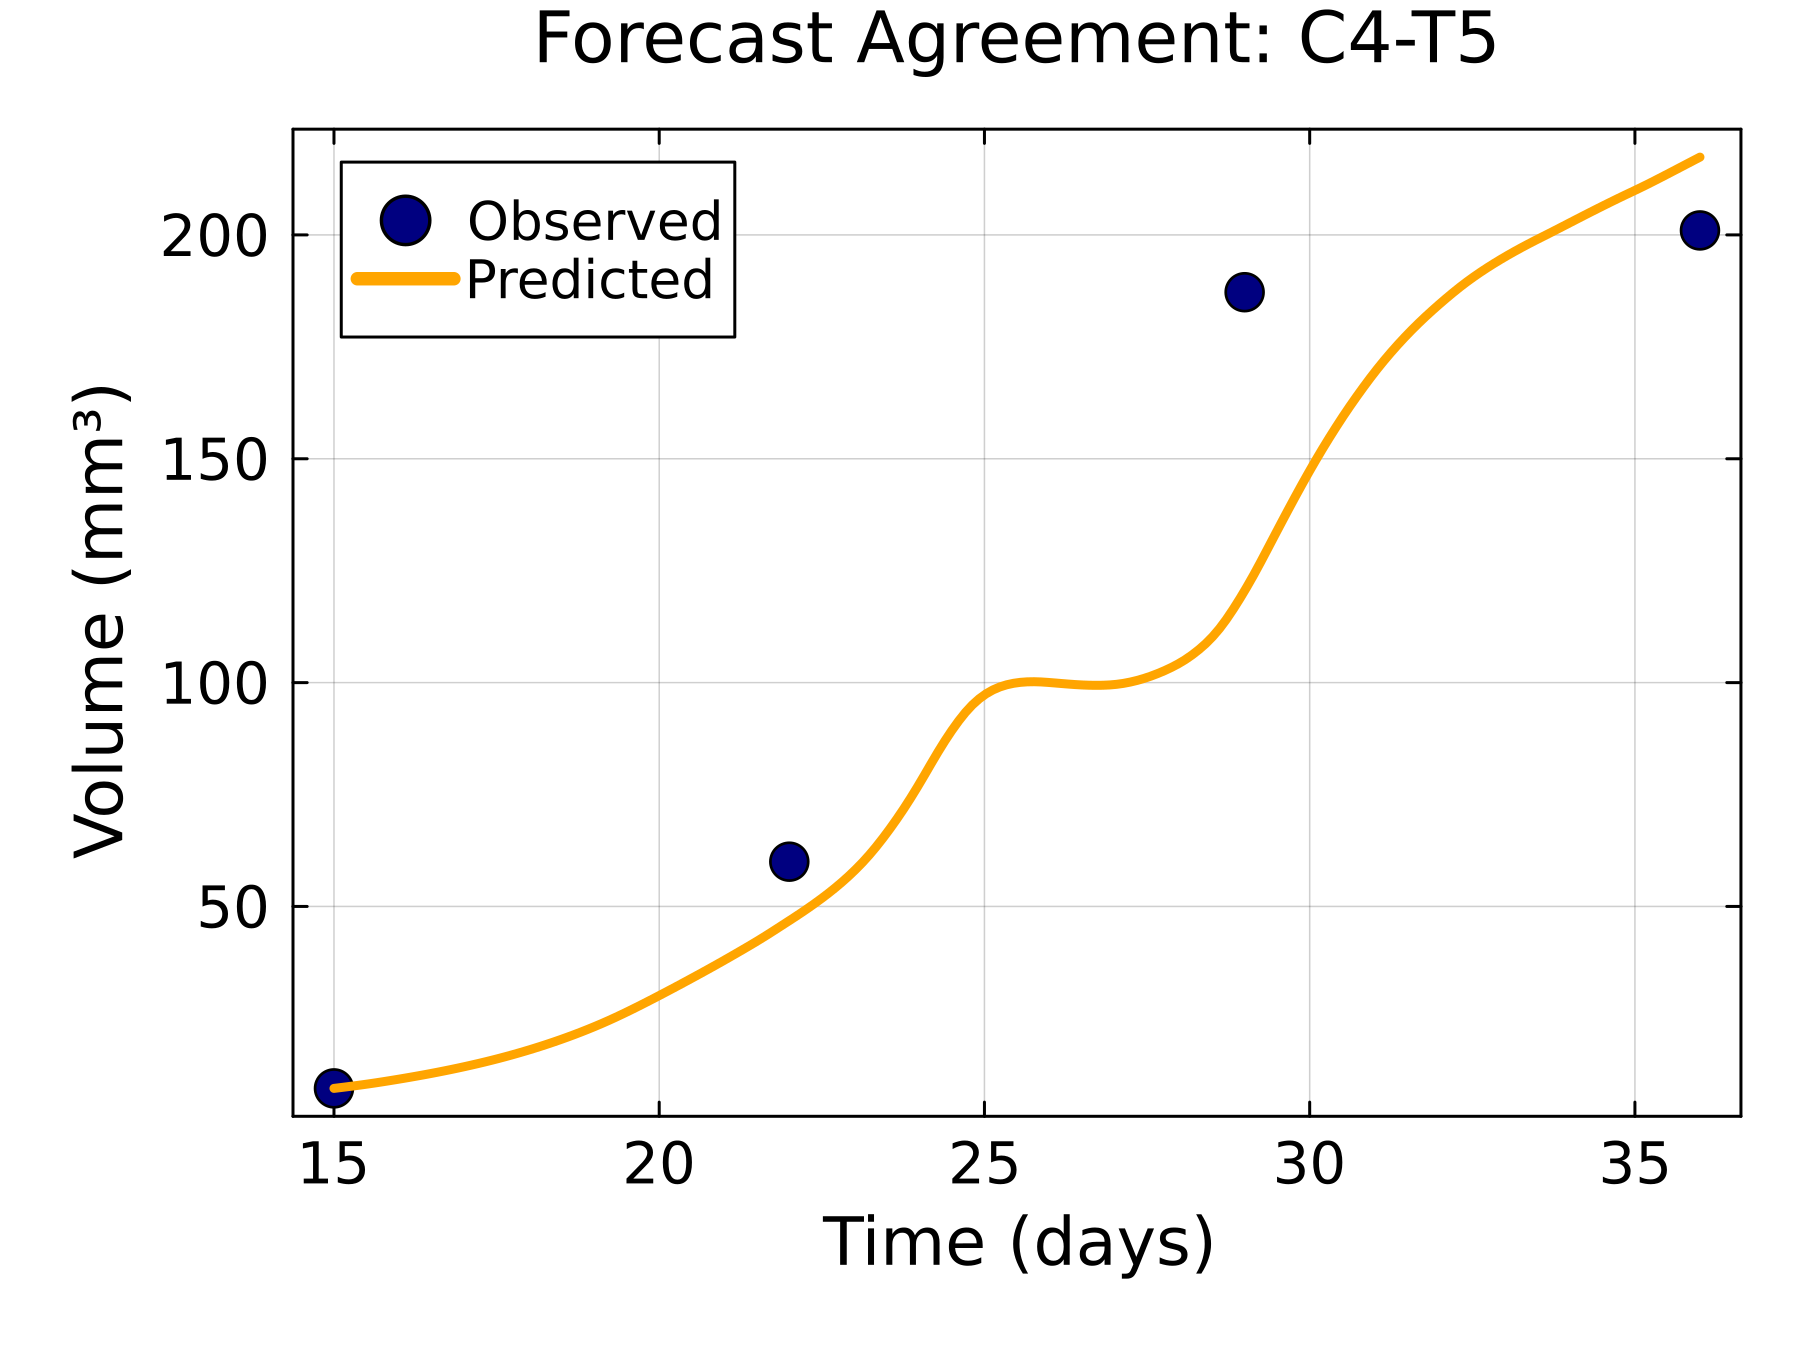
\includegraphics[width=\linewidth]{forecast_comparison.png}
\caption{Forecasting performance for C4-T5 showing agreement between observed and predicted volumes.}
\label{fig:c4t5_forecast}
\end{figure}

\begin{figure}[H]\centering
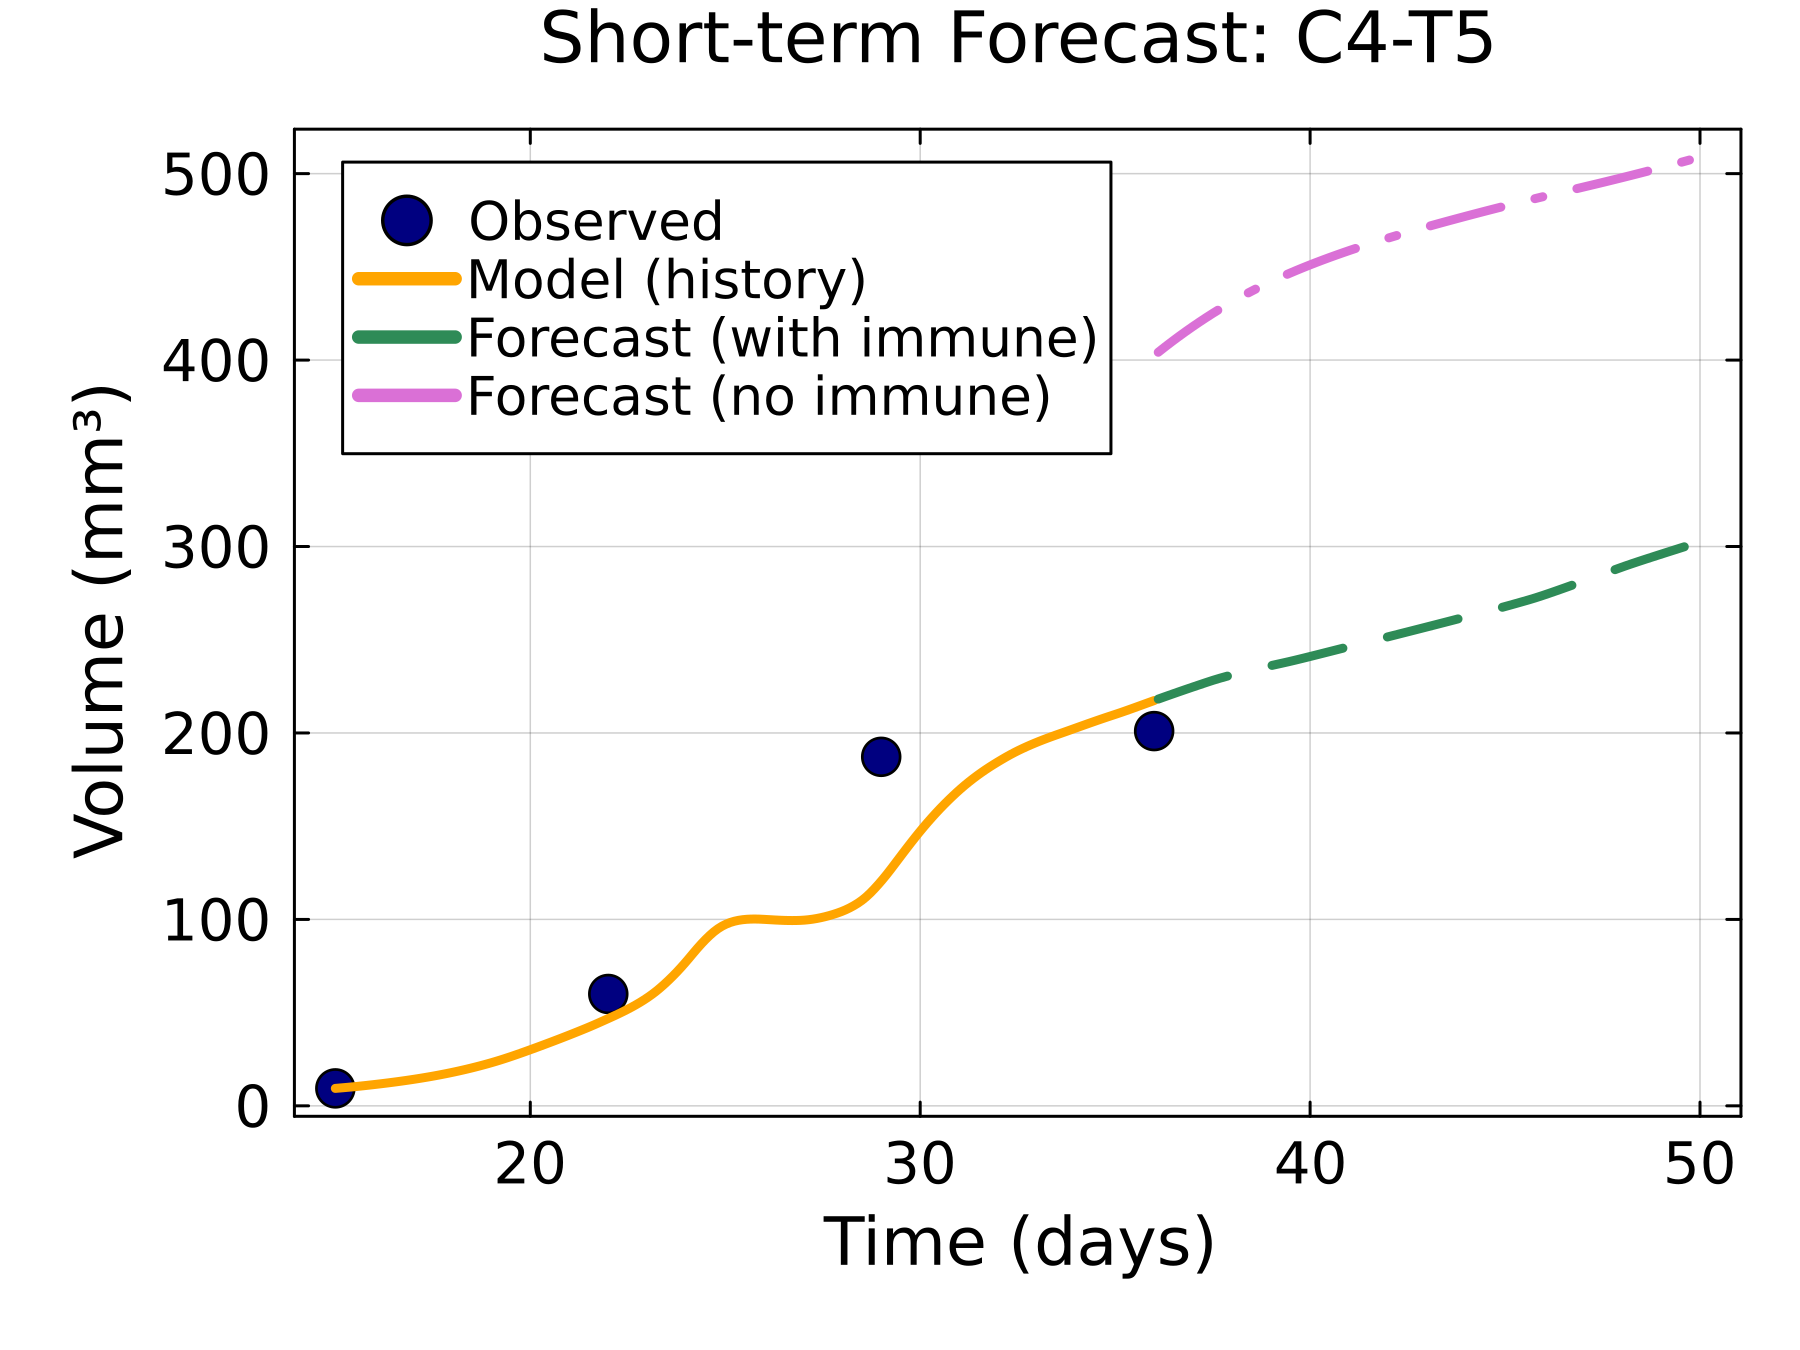
\includegraphics[width=\linewidth]{forecast_short.png}
\caption{Short-term (14-day) forecasting for C4-T5 with and without immune activity.}
\label{fig:c4t5_short_forecast}
\end{figure}

\begin{figure}[H]\centering
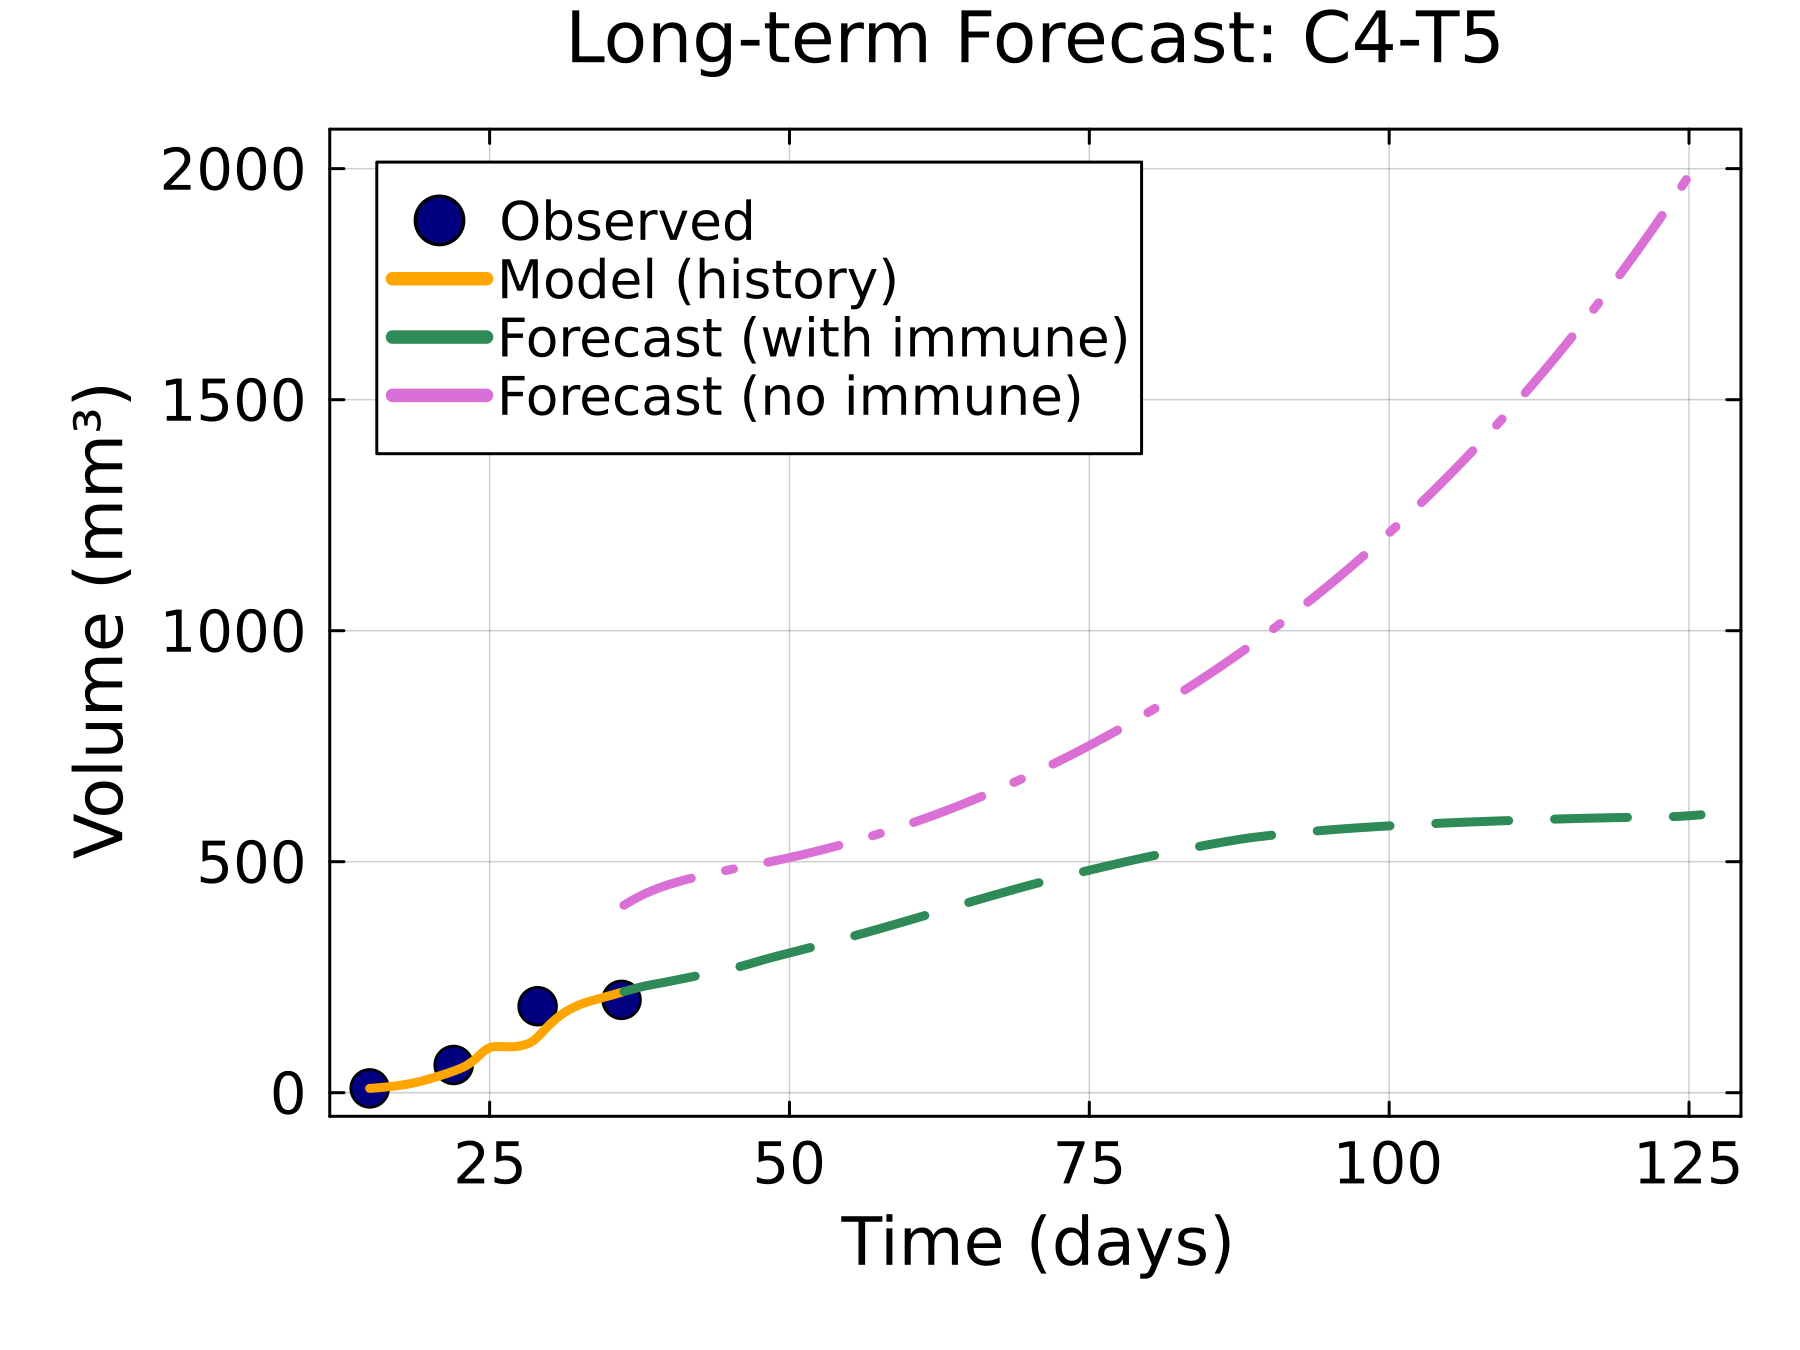
\includegraphics[width=\linewidth]{forecast_long.png}
\caption{Long-term (90-day) forecasting for C4-T5 with and without immune activity.}
\label{fig:c4t5_long_forecast}
\end{figure}

The temporal evolution of learned parameters (Figure~\ref{fig:param_trajectories}) shows how growth rates, carrying capacities, and immune parameters adapt over time, providing biological insight into tumor--immune interaction dynamics.

\begin{figure}[H]\centering
\includegraphics[width=\linewidth]{parameter_trajectories_history.png}
\caption{Parameter evolution trajectories for case C2-T1 showing temporal dynamics of $r(t)$, $K(t)$, $c_{\text{kill}}(t)$, and $h_{\text{sat}}(t)$.}
\label{fig:param_trajectories}
\end{figure}

\begin{figure}[H]\centering
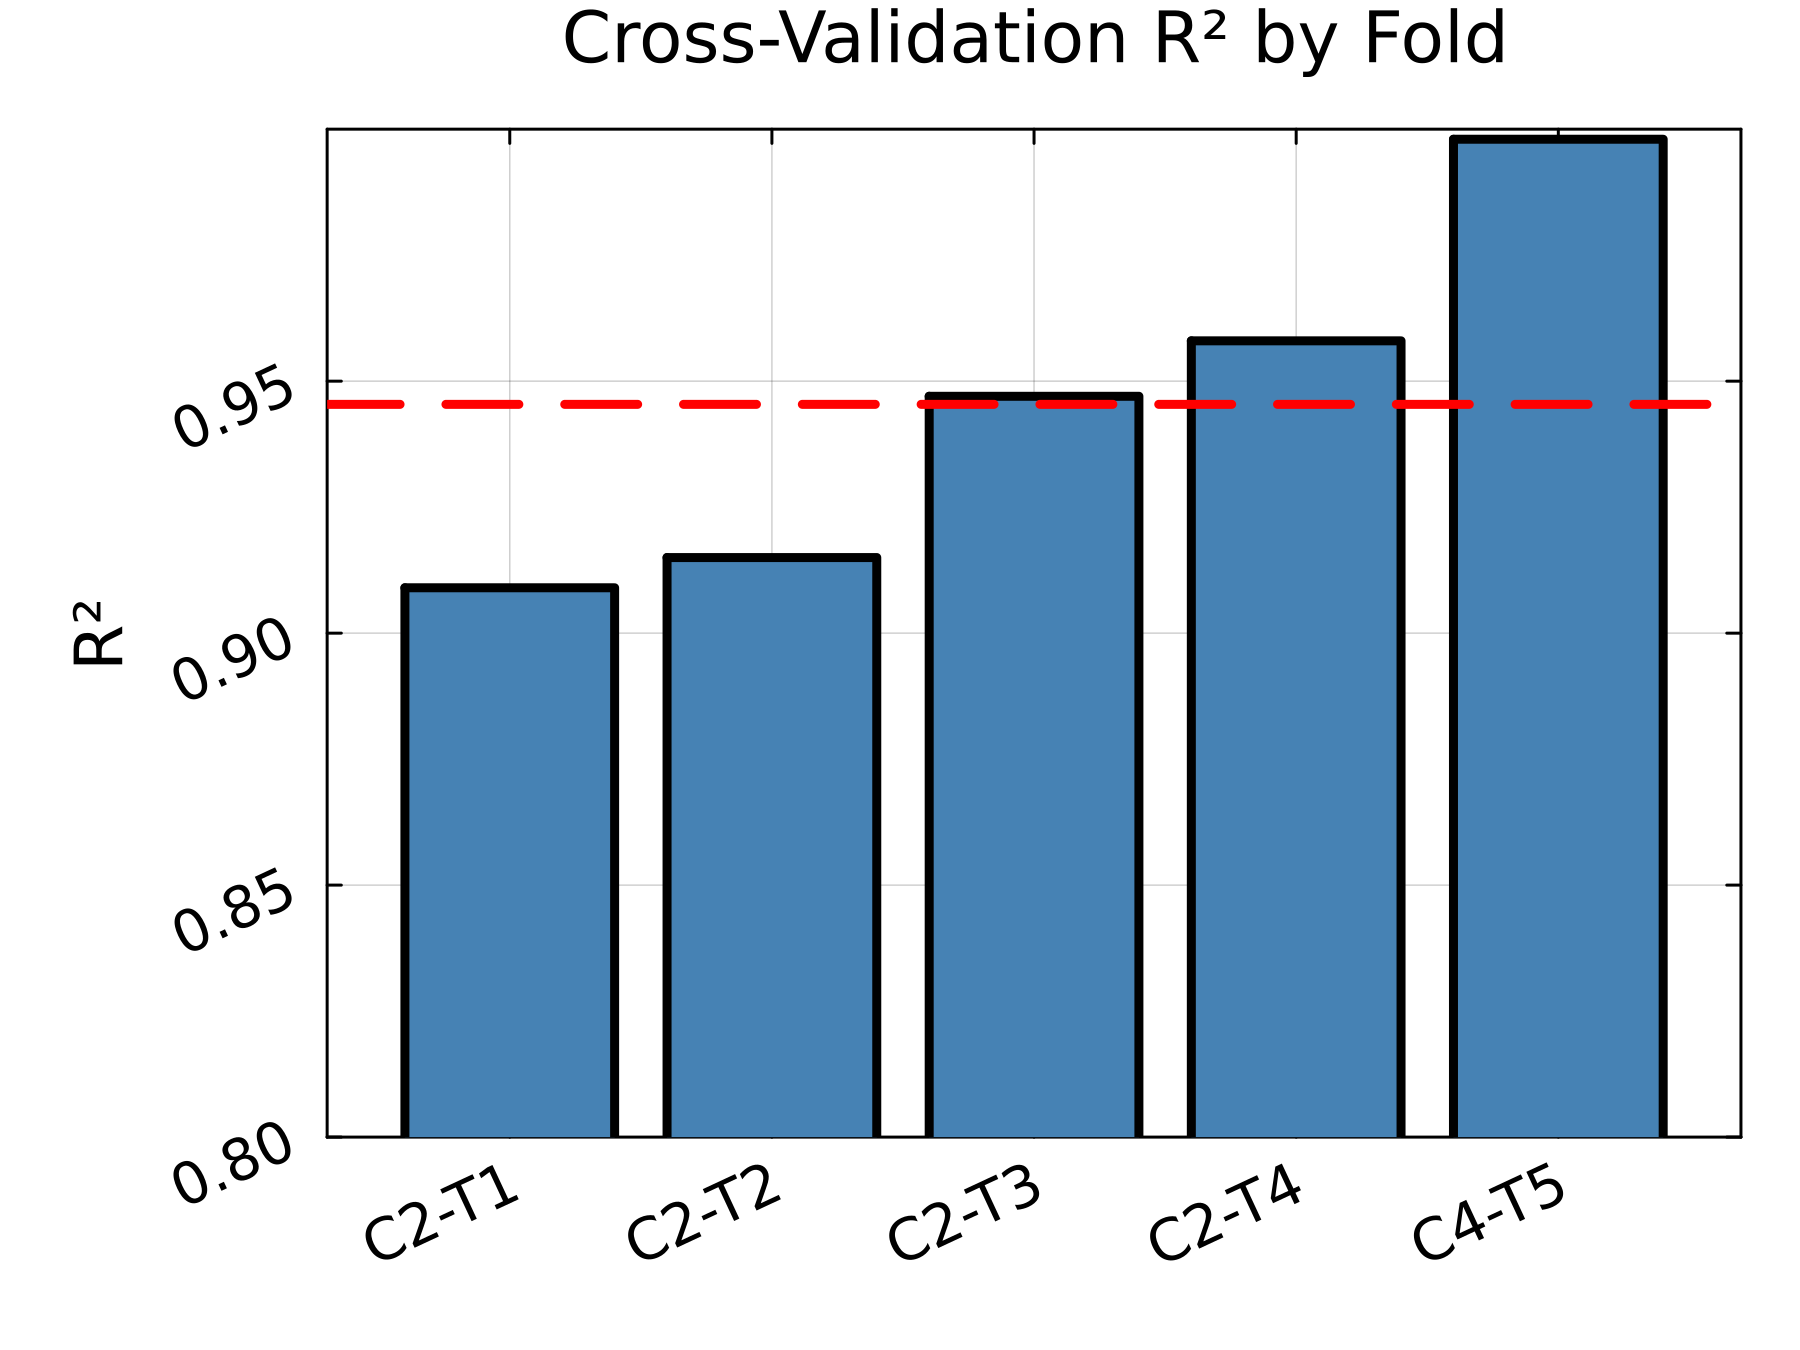
\includegraphics[width=0.8\linewidth]{r2_summary.png}
\caption{Distribution of $R^2$ values across cross-validation folds.}
\label{fig:r2_distribution}
\end{figure}

\begin{figure}[H]\centering
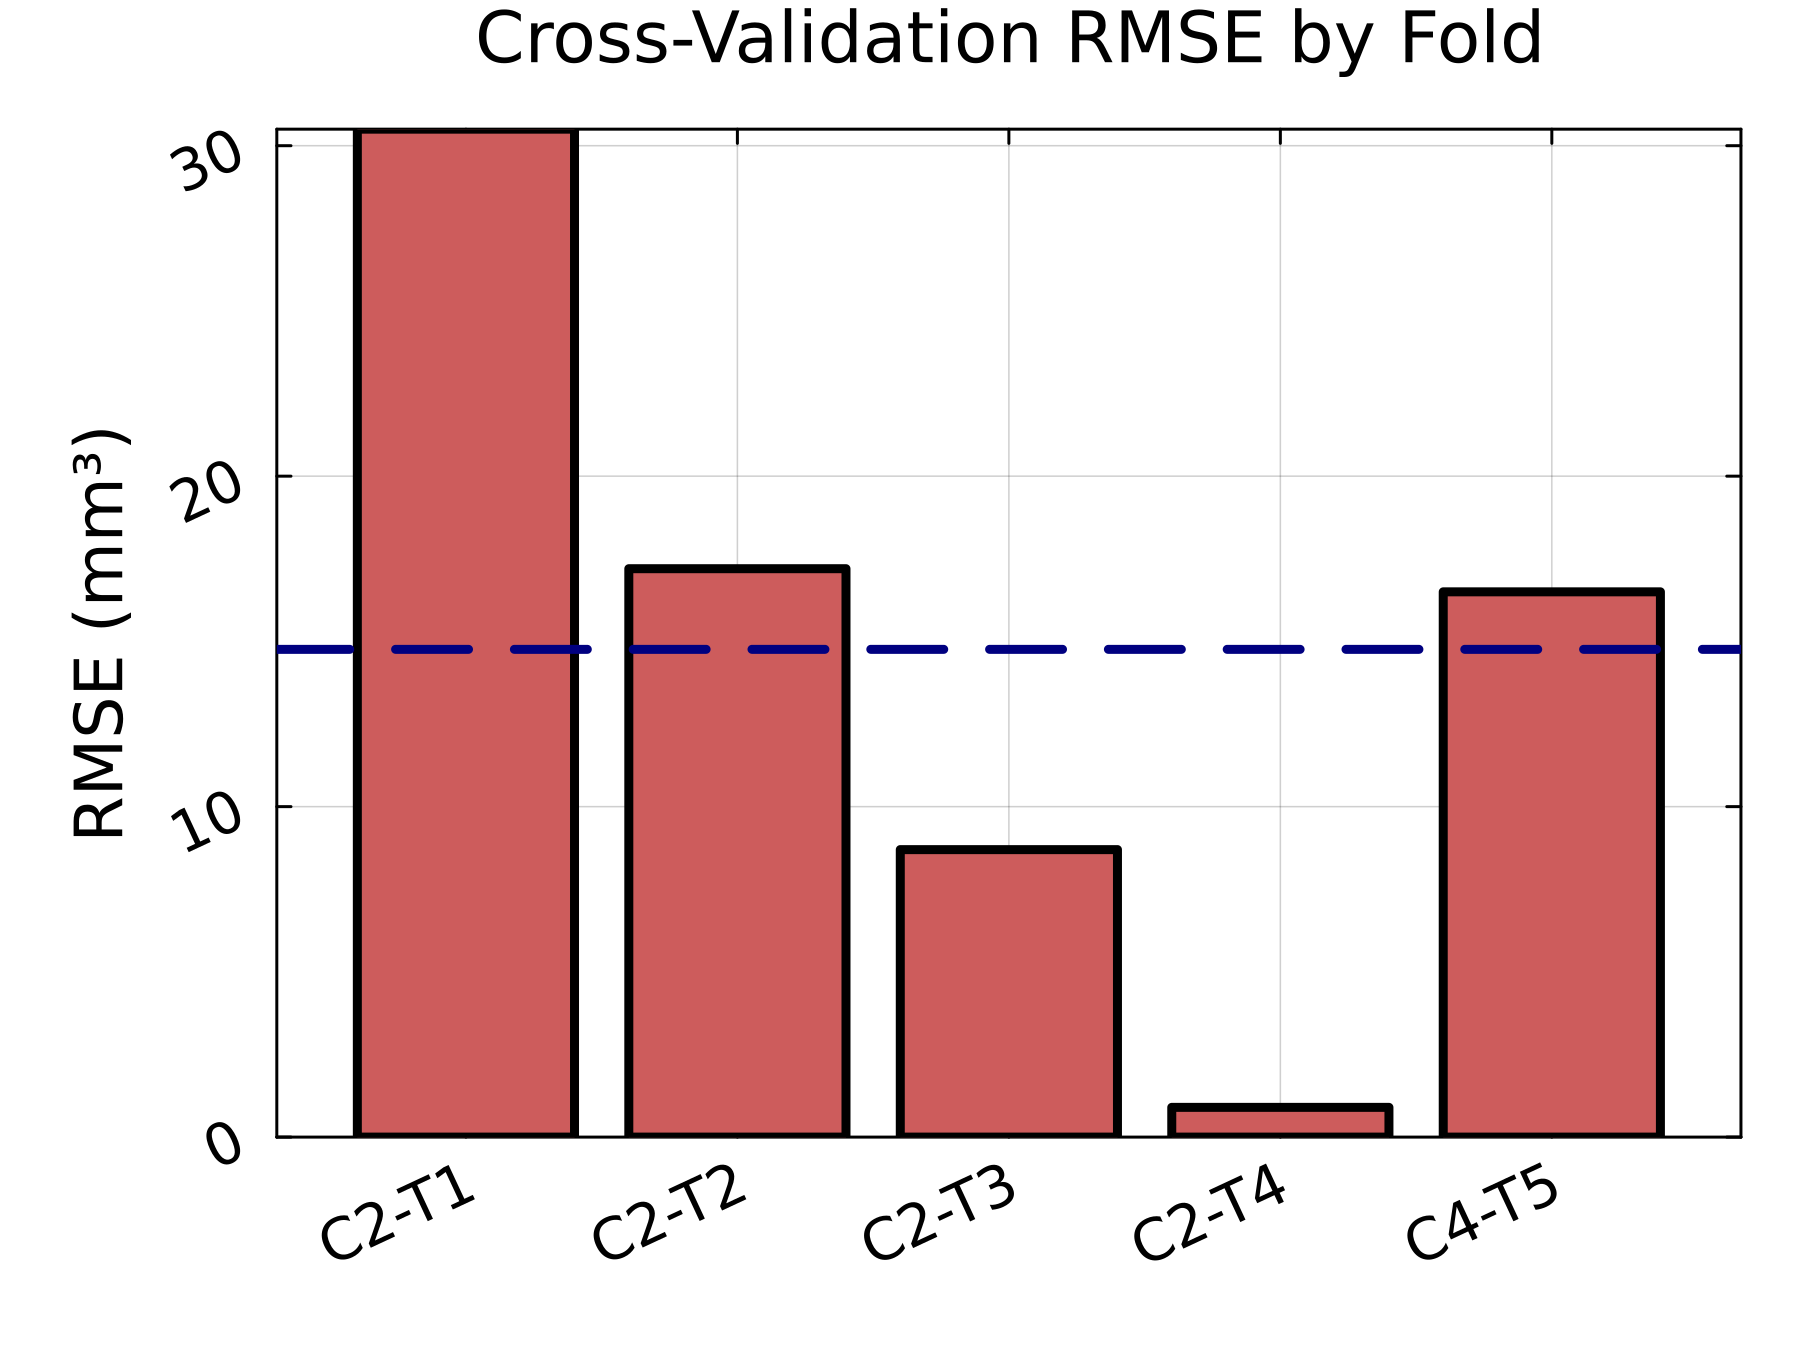
\includegraphics[width=0.8\linewidth]{rmse_summary.png}
\caption{Distribution of RMSE values across cross-validation folds.}
\label{fig:rmse_distribution}
\end{figure}

\subsection{Computational Performance}

Training takes 15--30 minutes per cross-validation fold on standard hardware (Intel i7, 16GB RAM). Inference is sub-millisecond per trajectory. Julia's SciML ecosystem provides efficient adjoint methods for gradient computation \cite{wang2023hybridizing,ramadhan2024data}.

% ===========================
\section{Discussion}

The progressive workflow from hybrid to structured-parameter UDE demonstrates a practical research pattern: the hybrid model's flexibility reveals what dynamics matter (complex immune responses, temporal corrections), while the structured-parameter model channels these insights into an interpretable framework. The structured-parameter UDE's higher accuracy ($R^2 = 0.991$ vs.\ $0.897$) suggests that constraining neural networks to output biologically meaningful parameters acts as effective regularization.

The cross-validation results (mean $R^2 = 0.945$) indicate reasonable generalization, though we note the dataset is small (five held-out groups from a single experimental system). The gap between training $R^2$ (0.991) and cross-validation $R^2$ (0.945) suggests some overfitting, which is expected given the model's expressiveness relative to dataset size.

From a software perspective, Julia's SciML ecosystem provides a cohesive development experience. The composability of DifferentialEquations.jl, Flux.jl, and SciMLSensitivity.jl enables rapid prototyping of UDE architectures, and the performance characteristics (sub-millisecond inference, efficient adjoint gradients) are well-suited to iterative model development.

\subsection{Limitations}
\label{sec:limitations}

This study has several important limitations that should be considered when interpreting the results.

\textbf{Limited baselines.} Our comparison includes only classical mechanistic ODE models (Gompertz, Kuznetsov--Taylor, de Pillis--Radunskaya). We do not compare against modern data-driven baselines such as Neural ODEs \cite{chen2018node}, latent ODE models \cite{dupont2019augmented}, or Gaussian process regression, which could provide competitive or superior performance on this dataset. Future work should include these comparisons to properly contextualize the UDE approach.

\textbf{No ablation studies.} We do not systematically ablate model components (e.g., removing individual loss terms, varying network size, testing different mechanistic backbones). Such studies would clarify which design choices contribute most to performance and are an important direction for future work.

\textbf{No uncertainty quantification.} Our models produce point predictions without confidence intervals. For any downstream application, uncertainty estimates are essential. Techniques such as ensemble methods, Monte Carlo dropout, or Bayesian neural network extensions could provide this, but are not implemented here.

\textbf{Naming and interpretability.} While we use the term ``structured-parameter'' to describe the Phase~2 architecture, it is important to note that neural networks learn all four biological parameters as functions of state. The model is not mechanistic in the traditional sense---it is a neural model whose outputs are structured through a mechanistic template. The biological interpretability of individual parameter trajectories should be treated with caution, as the neural networks may exploit the functional form in ways that do not correspond to true biological mechanisms.

\textbf{Dataset scope.} The dataset comes from a single experimental system with a small number of tumor--immune trajectories. Generalization to other tumor types, species, or experimental conditions has not been demonstrated. The single-compartment model also neglects spatial heterogeneity and metastatic dynamics.

\textbf{Forecasting caveats.} The reported forecasting metrics (MAPE of 1.8\% short-term, 4.3\% medium-term) are computed on this specific dataset and should not be interpreted as indicative of performance on independent datasets or in applied settings. Long-term forecasts beyond the training data's temporal extent are extrapolations and should be treated accordingly.

% ===========================
\section{Conclusions}

We have presented a progressive UDE workflow for tumor--immune dynamics modeling in Julia's SciML ecosystem. The dual-network hybrid UDE ($R^2 = 0.897$) serves as an exploratory tool, while the structured-parameter UDE ($R^2 = 0.991$, cross-validation mean $R^2 = 0.945$) demonstrates that channeling neural network outputs through classical equation structures can yield both high accuracy and parameter-level interpretability. The implementation showcases the capabilities of Julia's SciML ecosystem for composing differential equations with neural networks in a scientifically grounded manner. Important next steps include comparison against modern neural baselines, ablation studies, uncertainty quantification, and validation on larger and more diverse datasets.

% ===========================
\section{Research impact statement}
\label{sec:research-impact-statement}

This work demonstrates the application of Universal Differential Equations to tumor--immune dynamics modeling within Julia's SciML ecosystem. The progressive workflow from hybrid to structured-parameter models provides a replicable template for applying UDEs to biological systems. The physics-informed constraints and cross-validation framework contribute methodological tools that are transferable to other domains. The open-source implementation supports reproducible research in computational biology.

% ===========================
\section{AI usage disclosure}
\label{sec:ai-usage-disclosure}

AI-assisted tools (GitHub Copilot and Claude by Anthropic) were used during development for code assistance, debugging, and manuscript editing. All content was reviewed, verified, and revised by the author. The scientific methodology, experimental design, model architectures, and interpretation of results are the work of the author.

\bibliographystyle{juliacon}
\bibliography{ref}

\end{document}
